\documentclass[a4paper,12pt,oneside,bibtotoc,numbers=noenddot]{scrreprt}

%Pakete
\usepackage[latin9]{inputenc}
\usepackage[ngerman]{babel}

\usepackage{listings}
\usepackage{graphicx}

%\usepackage{makeidx}
%\makeindex


\usepackage{BachelorThesis}

% Allgemeine Informationen
\newcommand\mytitle{Titel der Arbeit}
\newcommand\myauthor{Name des Autors oder der Autoren}
\newcommand\mydepartment{Informatik und Elektrotechnik}
\newcommand\myinstitute{Hochschule Zittau/G\"{o}rlitz}
\newcommand\mytutor{Name und Titel des betreuenden Professors}
\newcommand\mySecondTutor{Name und Titel des betrieblichen Betreuers}

% Abstracts
\newcommand\mysubject{Das deutsche Abstract.}
\newcommand\mysubjectenglish{The english abstract.}

% PDF-Einstellungen
\hypersetup
{
	pdftitle = \mytitle,
	pdfsubject = \mysubject,
	pdfauthor = \myauthor,
	pdfkeywords = {},
	colorlinks = {true},
	pdfborder = 0 0 0
}


\begin{document}
\nocite{*}


%
\pagenumbering{alph}
\begin{titlepage}
\thispagestyle{empty} 
 \begin{center}
 {\bfseries \LARGE Teil 1\\}
 {\bfseries \huge Das Wohnheimprojekt \\} 
 \vspace{1cm}
 {\bfseries \LARGE Teil 2\\}
 {\bfseries \huge Das Projekt Datenbankkonfigurationen\\}
 \vspace{1.0cm} 
 {\bfseries \huge Belegarbeit\\}
 \vspace{1.0cm}
 {\normalsize eingereicht am Fachbereich\\}
 {\bfseries \Large Informatik\\}
 {\normalsize der Hochschule Zittau/G�rlitz (HAW)\\}
 \vspace{1cm}
 {\normalsize als Pr�fungsleistung im Fach\\}
 {\bfseries \Large Fortgeschrittene Datenbank-Konzepte 1\\}
 \vspace{1cm}
 {\normalsize vorgelegt von:\\}
 {\bfseries \Large Christof Ochmann (35989)\\
 Stefan L�ttke (43053) \\
 Ingo K�rner (40586)\\}
 \vspace{1cm}
 {\normalsize  G�rlitz, 3. Februar 2012\\}
 \vspace{0.5cm}
 Betreuer:	Prof. ten Hagen\\
 \vfill
\end{center}
\end{titlepage}

%

%% Kurzreferat
\thispagestyle{empty}
\section{Abstract}\label{Abstract}
Diese Arbeit besch�ftigt sich damit, wie sich die Performance von Abfragen steigern l�sst. Dabei wird nur der Bereich OLAP betrachtet. Der Datenimport mit Load sowie der Bereich OLTP werden nicht untersucht. Es wird nur auf Kaltstarts eingegangen, wie sie im Bereich Datawarehouse vorkommen. Performancesteigerungen mittels Caching bei Warmstarts sind nicht Gegenstand dieser Arbeit. Es wird untersucht, wie sich verschiedene Arten von Indexen und verschiedene Arten des Partitionings auf die Abfrageperformance von SQL-Queries auswirken. F�r die empirischen Messungen der Performance wird exemplarisch das Szenario eines Onlineshops gew�hlt, indem die Verk�ufe analysiert werden.\\
Diese Arbeit beantwortet die Frage, welche Datenbankkonfiguration f�r die gew�hl\-ten SQL-Abfragen im Durchschnitt die h�chste Abfrageperformance leistet. Ziel der Arbeit ist, Annahmen �ber die Performance verschiedener Konfigurationen zu treffen, diese theoretisch zu begr�nden und dann durch Messergebnisse praktisch zu belegen. Anhand von Messergebnissen werden die aufgestellten Hypothesen best�tigt oder wiederlegt. F�r wiederlegte Hypothesen wird eine Begr�ndung gesucht. Es wird davon ausgegangen, dass verschiedene Indexarten einen unterschiedlichen Einfluss auf bestimmte Queries haben werden. Es wird gezeigt, bei welchen Queries welche Indexarten bei welchen Spalten die Ausf�hrungszeit beschleunigen. Es wird angenommen, dass verschiedene Partitionierungsarten einen unterschiedlichen Einfluss auf bestimmte Queries haben werden. Es wird gezeigt, bei welchen Queries welche Partitionierungsarten auf welchen Spalten die Ausf�hrungszeit beschleunigen.\\
�ber die Ergebnisse der Arbeit l�sst sich zusammenfassend sagen, dass Hashindexe auf Prim�r- und Fremdschl�ssel die Abfragen im Durchschnitt um Faktor x beschleunigen, gegen�ber dem Weglassen s�mtlicher Indexe. Wird dar�ber hinaus X-Partitioning verwendet, beschleunigt das die Abfragen im Durchschnitt nochmal um Faktor x, gegen�ber der reinen Verwendung von Indexen. Wird dar�ber hinaus sogar ein Subpartitioning verwendet, beschleunigt das die gew�hlten Abfragen im Durchschnitt um Faktor x, gegen�ber der Verwendung von Partitions mit Indexen.

%\mysubject
%\section*{Abstract}
%\mysubjectenglish

\pagenumbering{Roman}
\tableofcontents
\listoffigures
\lstlistoflistings

\begin{listofacronyms}
\acronym{API}{Application Programming Interface}
\acronym{ACID}{Atomicity, Consistency, Isolation, Durability}
\acronym{BLOB}{Binary Large Object}
\acronym{DBMS}{Database management system}
\acronym{ERD}{Entity-Relationship Diagram}
\acronym{IDE}{Integrated Development Environment}
\acronym{JDK}{Java Development Kit}
\acronym{MyISAM}{My Indexed Sequential Access Method}
\acronym{OLAP}{Online Analytical Processing}
\acronym{OLTP}{Online Transaction Processing}
\acronym{PHP}{Hypertext Preprocessor}
\acronym{SQL}{Structured Query Language}
\acronym{WLAN}{Wireless Local Area Network}

\end{listofacronyms}

\begin{flushleft}
\begin{thebibliography}{sotief}
\bibitem{bib1}{Martin, Robert C. (2008): Clean Code: A Handbook of Agile Software Craftsmanship. Prentice Hall International}

\bibitem{bib2}{Freeman, Eric (2007): Entwurfsmuster von Kopf bis Fu�. O'REILLY}

\bibitem{bib3}{\begin{verbatim}http://www.easymock.org/EasyMock3_0_Documentation.html
Abruf: 21.12.2011\end{verbatim}} 

\bibitem{bib4}{\begin{verbatim}http://dev.mysql.com Abruf (11.01.2012)\end{verbatim}} 
\bibitem{bib5}{D��ler, Rolf (2011): MySQL. bhv}
\bibitem{bib6}{Schwartz, Baron. (2008): High Performance MySQL. O'REILLY}
\bibitem{bib7}{\begin{verbatim}http://code.google.com/p/google-guice Abruf: 11.01.2012\end{verbatim}} 

\end{thebibliography}
\end{flushleft}



\newpage
\pagestyle{chapterStyle}
\pagenumbering{arabic}

\part{Das Projekt Wohnheimdatenbank}
\chapter{Projekt Wohnheimdatenbank}
\section{Problemstellung}
Anfangs war die Idee, eine Erweiterung der bestehenden Datenbank der Wohnheime Vogtshof und Hirschwinkel durch ein Datenbankschema, welches Informationen dar�ber enth�lt, welche IP-Adresse von welchem Mieter wann benutzt wurde und wird. Dies sollte der R�ckverfolgung von verd�chtigen Aktivit�ten dienen, welche bereits in der Vergangenheit lagen und vom derzeitigen System nicht mehr dargestellt werden k�nnen. Die Informationen sollten �ber die Zeit gesammelt und archiviert werden. Im n�chsten Schritt sollten die Informationen �ber das bereits bestehende Web-Interface eingesehen werden k�nnen. Dazu war geplant eine kleine Suchfunktion zu implementieren, welche es erlauben sollte, die Geschichte f�r eine bestimmte IP abrufen zu k�nnen.

\section{Planung}
Es wurde sich f�r ein eigenst�ndiges Datenbankschema entschieden, da es kritisch werden k�nnte, wenn man an dem bestehenden Live-System arbeiten w�rde. Um sicher zu gehen, das die Daten auch korrekt und zum richtigen Zeitpunkt eingetragen werden sollte mit Triggern gearbeitet werden, die immer ausgel�st werden sollten, wenn eine IP vergeben wurde. Der genaue Aufbau kann den nachfolgenden Grafiken entnommen werden

Anmerkung des Authors: Grafiken m�ssen noch generiert werden!!!

Ein Problem bei der Planung waren die Unterschiedlichen Wege an eine IP zu kommen. Da ein Mieter nicht zwingend einen Administrator aufsuchen muss um eine vorr�bergehende IP zu bekommen, w�re die alleinige Nutzung von Triggern nicht ausreichend gewesen.
Eingesetzte Technologien
Da dieses Projekt nicht als komplettes Refactoring bzw. �berarbeitung der bereits bestehenden Software gedacht war mussten die bereits eingesetzten Technologien genutzt werden. Auf der Datenbank musste daher PostgreSQL zum Einsatz kommen. Als Hochsprache w�re zudem PHP genutzt worden.

\section{Juristische und moralische �berlegungen}
Die Theoretische Ausarbeitung Planung war damit abgeschlossen. Da sich dieses Projekt jedoch in einer Grauzone des Datenschutzes bewegte mussten noch weitere moralische und juristische Dinge abgewogen werden. Durch den Einsatz der Softwareerweiterung w�ren s�mtliche Mieter der beiden G�rlitzer Wohnheime unter Generalverdacht geraten. Auf der anderen Seite w�re es Ermittlungsbeh�rden damit m�glich gewesen ohne gro�e B�rokratie den Namen eines Verd�chtigen zu erfahren, wenn sie nur Zugang zu dessen IP gehabt h�tten. Dieses Argument mag bei relativ geringf�gigen Verbrechen wie illegalen Down- oder Uploads noch keine hohe Bedeutung haben. Sobald wir uns jedoch in einem Bereich befinden in dem Menschen zu Schaden kommen ist es erstrebenswert die entsprechenden T�ter schnell zu ermitteln.\\
Doch die T�ter zu ermitteln ist in einem Rechtsstaat nicht ausreichend. Selbst wenn mit Hilfe unserer Datenbankerweiterung ein T�ter gefasst worden w�re, bliebe die Frage offen, ob die Informationen auch juristisch verwertbar w�ren. Dazu h�tte man beweisen m�ssen, dass die zur Verf�gung gestellten Informationen nicht manipulierbar gewesen w�ren. Um dies zu beweisen h�tte sichergestellt werden m�ssen, das sich niemand die angeforderte IP �ausgeborgt� hat. Dies ist jedoch weitestgehend unm�glich, da es verschiedene Wege g�be sich eine Fremde IP im Wohnheimnetzwerk zu besorgen. Als Beispiel k�nnte hier das �ndern der Mac-Adresse genannt werden. Bei Nutzern mit einem WLAN-F�higen Router w�re auch das Eindringen in deren interne Netzwerk m�glich gewesen.\\
All diese Fakten mussten nun abgewogen werden. Die Letzte Entscheidung hatten jedoch die Vertreter des �Studentwerk Dresden�, welche den Schutz der Pers�nlichkeitsrechte ihrer Mieter als wichtiger und die M�glichkeit des Missbrauchs der Daten als zu gef�hrlich ansahen. Dieser Meinung schloss sich auch ein Gro�teil des Teams an, was neben den oben erw�hnten technischen Problemen dazu f�hrte das das Projekt beendet werden musste.


\part{Das Projekt Datenbank\-konfigura\-tionen}


\chapter{Theorie}
\section{Einleitung}\label{einleitung}
Ziel dieses Projektes ist die Performance eines relationalen Datenbankmagagementsystems f�r bestimmte Konfigurationen zu testen. Die Konfiguration ergibt sich aus den Anforderungen, die an das DBMS bzw. die konkrete Datenbank gestellt werden. 
Es ergibt sich die Frage, f�r welche konkrete Anforderung welche konkrete Konfiguration gew�hlt werden sollte? Um diese Frage zu beantworten, sind mehrere Schritte n�tig. Es wird zuerst ein DBMS exemplarisch ausgew�hlt. Dann wird f�r dieses DBMS ein ERD angefertigt, dass die Tabellen beschreibt. Um die Performance zu testen, muss ein Datengenerator geschrieben werden, der die Testdaten f�r die Tabellen generiert. Die konkreten Anforderungen, die an den Datengenerator gestellt werden, m�ssen analysiert werden. Dann wird der Generator entworfen, implementiert und getestet. F�r den Datengenerator wird ein Build Mangagement Tool eingesetzt sowie Frameworks f�r Dependency Injection und zum Testen der Anwendung. Dann werden f�r die Konfigurationen Queries auf den mit Testdaten bef�llten Tabellen gefahren und die Antwortzeiten gemessen. Die Messungen erfolgen alle auf einem Referenzsystem. So k�nnen verschiedene Konfigurationen �ber ihre Performancewerte miteinander verglichen werden.
\section{Aufgabenstellung}\label{Aufgabenstellung}
In diesem Projekt soll die Abfrage-Performace f�r ein bestimmtes Szenario gemessen werden. Dazu ist ein Szenario auszuw�hlen, das im Bereich OLAP und Data Warehouse angesiedelt ist. F�r das Szenario sind geeignete Konfigurationen zu w�hlen. Konfigurationen unterscheiden sich in Art- und Anzahl von Indexen und in den Partitionierungsarten. Es wird angenommen, dass jede Konfiguration f�r eine bestimmte Art von Abfragen besonders geeignet ist. Es sollen verschiedenartige Abfragen gew�hlt werden, f�r die jeweils die Performance gemessen wird. Um die Performance messen zu k�nnen, ist ein ERD f�r ein gew�hltes Szenario anzufertigen. Die Tabellen des ERD sollen mit Testdaten gef�llt werden. Dazu ist ein Datengenerator anzufertigen. Die Abfragen werden auf die gef�llten Tabellen angewendet. Die Zeit, die ein Query braucht, um auf einer bestimmten Konfiguration ausgef�hrt zu werden, wird gemessen. Das Messergebnis wird mit der Annahme verglichen und ausgewertet.
\section{Relevanz des Forschungsgegenstandes}\label{RelevanzDesForschungsgegenstandes}
Der Forschungsgegenstand in dieser Arbeit ist es, geeignete Konfigurationen f�r verschiedene, konkrete, praxisrelevante Anwendungsf�lle zu finden. \\
Der Forschungsgegenstand ist relevant, da bisher keine konkreten Werte, die die Performance der gew�hlten Konfigurationen beschreibt, vorliegen. Ziel dieser Foschung ist es, die Annahmen f�r Konfigurationen zu treffen, die Performance der Konfigurationen zu messen und dann zu interpretieren, ob die Annahmen sich mit den Messergebnissen best�tigen oder wiederlegt werden. Die Herausforderung dieser Arbeit ist, geeignete Anwendungsf�lle aus verschiedenen Anforderungen von Anwendungen zu finden. F�r jede dieser Anwendungsf�lle die geeignetste Kongiguration zu w�hlen. F�r diese Konfiguration werden dann Annahmen getroffen und Performancewerte gemessen. Die Annahmen werden dann mit Hilfe der Messergebnisse verifiziert bzw. falsifiziert. Um die Performance von Konfigurationen messen zu k�nnen, muss ein Testdatengenerator angefertigt werden. Dabei m�ssen technische Probleme gel�st werden. Um die optimale Konfiguration f�r einen Anwendungsfall zu finden, muss sich vertiefend in eine Datenbanken eingearbeitet werden. Das geschieht z.B. unter Zuhilfenahme von B�chern und Online-Ressourcen. In diesen Medien ist der Forschungsstand zur Erstellung von Konfigurationen dokumentiert.
\section{Der aktuelle Wissensstand}
Vorhandene Kenntnisse �ber die Erstellung von Konfigurationen werden haupt\-s�chlich aus Onlineressourcen bezogen. Bei der Umsetzung der Anforderungen wird aus mehreren L�sungsm�glichkeiten jeweils die am besten geeignete ausgew�hlt und die Wahl wird begr�ndet. Prim�rliteratur zur gew�hlten Datenbank ist unter www.XXX.de zu finden. Unter dieser Adresse ist das gew�hlte DBMS dokumentiert. Auf dieser Seite wird eine Einf�hrung in XXX gegeben. Es gibt Installationsanleitungen, Programmier-Tutorials, eine umfassende Dokumentation von XXX und Werkzeuge die ein effizienteres Arbeiten mit XXX erm�glichen.
\section{Anwendungsf�lle f�r Datenbankanwendungen}\label{AnwendungsfaelleFuerDatenbankanwendungen}

\begin{itemize}
\item \textbf{Anwendungsfall 1}\\
Ein Online-Shop will seine Bestellungen �ber eine MySQL-Datenbank abwickeln. (innoDB)

\item \textbf{Anwendungsfall 2}\\
Das Management des Online-Shops m�chte Abfragen auf bestimmten Tabellen t�tigen, wie z.B.:

\begin{itemize}
\item Welches Produkt wurde wie oft gekauft?
\item Wieviel Umsatz wurde von wem in einem bestimmtem Zeitraum generiert?
\item Wie viele Kunden haben in einem bestimmten Zeitraum bestellt?
\end{itemize}

Dabei soll die Antwortzeit auch bei Queries �ber alle Daten nicht l�nger als eine Sekunde dauern. (Memory)

\item \textbf{Anwendungsfall 3}\\
Ein bekannter Blogger m�chte das Weblog-System WordPress einsetzen um Beitr�ge zu ver�ffentlichen. Die Kommentare und Blog-Posts werden strukturiert gespeichert. Zu bestimmten Spitzenzeiten laden hunderte Leser gleichzeitig seine Blogposts. (MyISAM)

\item \textbf{Anwendungsfall 4}\\
In einer Erdbebenwarnstation sollen Bodenersch�tterungen durch einen Seismografen erfasst und digital archiviert werden. Der Seismograf misst 50 mal in der Sekunde. Es sollen auch feinste Amplitudenausschl�ge erfasst werden. (Archive)
\end{itemize}
\section{Projektplanung}
\subsection{Datenbank}

\begin{figure}[h]
	\centering
		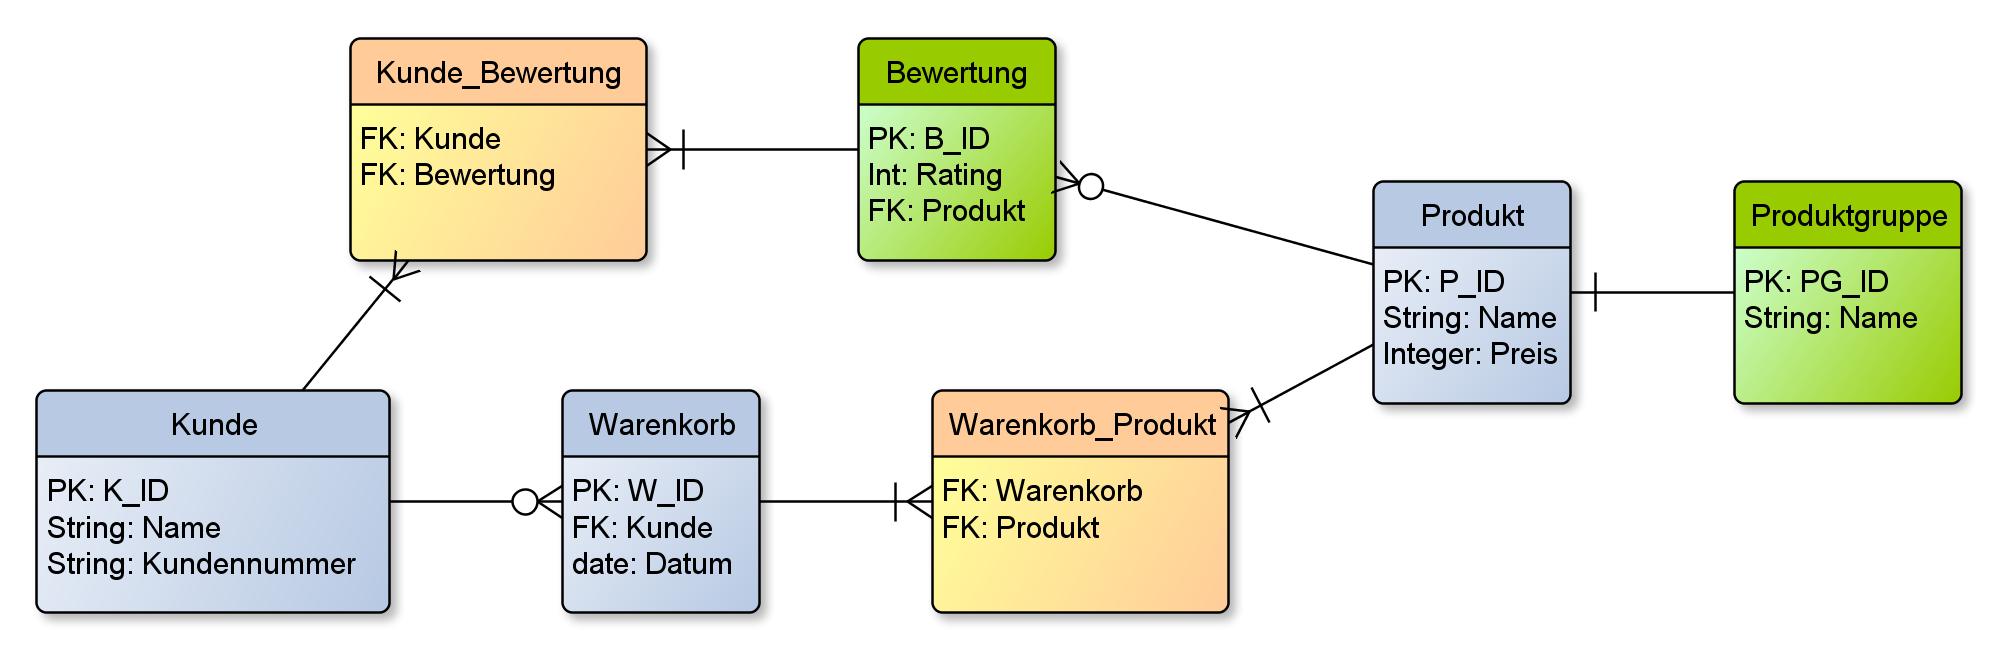
\includegraphics[width=1.0\textwidth]{Steff/ADBC-ERD.png}
	\caption{Orginal-ERD}
	\label{fig:ADBC_ERD}
\end{figure}

Das ERD beschreibt die Architektur unserer Datenbank. Die urspr�ngliche Planung sah vor, dass die Datenbank bei ausreichender Zeit noch erweitert werden konnte um mehr Anwendungsf�lle simulieren zu k�nnen. In diesem Fall w�ren die Tabellen die gr�n markiert sind, sowie die angrenzenden Verbindungsverbindungstabellen(rot markiert) zus�tzlich erstellt worden.
Die Tabellen mit der h�chsten Priorit�t waren aber Kunde, Warenkorb und Produkt. Dadurch wurde das Datenmodell, welches letzten Endes erstellt wurde �u�erst kompakt.\\
Anm.: Grafik wird noch generiert\\
Da es in MySQL nicht ohne weiteres m�glich ist die Indexe f�r die Versuche zu entfernen, wurden zwei Datenmodelle erzeugt, welche jeweils miteinander kompatibel sind. Dadurch waren wir in der Lage die Versuche relativ schnell hintereinander zu absolvieren. Au�erdem konnte so eine Optimierung der Zeiten f�r die 'Inserts' erreicht werden.
\subsection{Datenbankabfragen}
\begin{figure}[h]
	\centering
		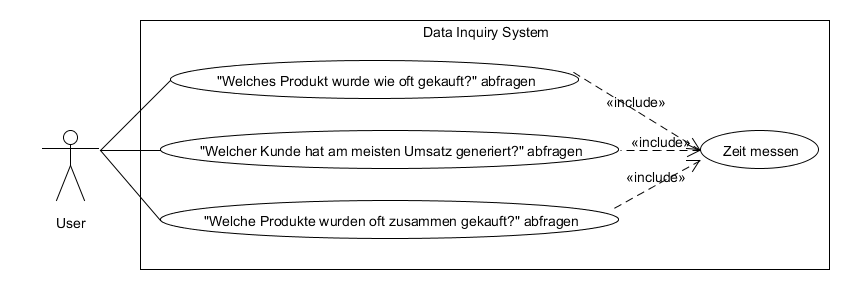
\includegraphics[width=1.0\textwidth]{Steff/UC.png}
	\caption{Datenbankabfragen}
	\label{fig:AbfragenUC}
\end{figure}
Da unser Projekt einen Webshop imitieren sollte, haben wir unsere Anwendungsf�lle so gew�hlt, wie sie auch in der Realit�t gefunden werden k�nnen. Sie k�nnten unter anderem Managern bei der Auswertung ihrer Gesch�fte dienen. Das gesamte Spektrum an m�glichen Abfragen abzudecken, h�tte jedoch den Zeitrahmen extrem gesprengt. Deshalb wurde sich f�r die folgenden drei Abfragen entschieden:
\begin{itemize}
	\item Welches Produkt wurde wie oft gekauft?
	\item Wie viel Umsatz wurde von wem in bestimmtem Zeitraum generiert?
	\item Wie viele Kunden haben in bestimmten Zeitraum bestellt? 
\end{itemize}
Diese Abfragen haben unterschiedliche Komplexit�ten. So m�ssen bei der zweiten Abfrage s�mtliche Tabellen einbezogen werden, w�hrend bei der ersten Abfrage nur zwei Tabellen involviert sind.
Auf diese Weise soll ein m�glichst breites Spektrum an Abfragen getestet werden, um sicher zu stellen, dass die Versuche so aussagekr�ftig wie m�glich werden.
\section{Eingesetzte Datenbanken}
W�hrend der Arbeiten am Projekt musste entschieden werden welche  Datenbank benutzt werden sollte. Um dies zu entscheiden orientierten wir uns zun�chst an der Vorlesung, da wir in der darin genutzten Datenbank sicher sein konnten, dass s�mtliche ben�tigten Funktionen enthalten waren. Diese Datenbank war Oracle SQL. Eine andere Datenbank, auf die wir sp�ter erst ein Auge geworfen haben war MySQL, da sie neben der Oracle SQL ebenfalls alle n�tigen Funktionen enthielt.
\subsection{Oracle SQL}
Die erste Datenbank mit der wir gearbeitet haben war Oracle. Da sie bereits in der Vorlesung vorgestellt wurde. Es gibt sie in zwei Versionen:

\begin{itemize}
	\item Die kostenfreie Express-Version
	\begin{itemize}
		\item Unbegrenzt nutzbar
		\item Eingeschr�nkte Funktionen
		\item Leicht zu installieren
	\end{itemize}
	\item Die kostenpflichtige Enterprise-Version
	\begin{itemize}
		\item o	Nutzung ohne Lizenz auf 30 Tage begrenzt
		\item Voller Funktionsumfang
		\item Komplizierte Installation 
\end{itemize}


\end{itemize}
Beide Versionen konnten von uns genutzt werden, da man in der Express-Version bereits das Datenbankschema und die Abfragen zusammenstellen und testen konnte, bevor man sie in der Enterprise-Version mit Partitioning erg�nzt. So war es m�glich etwas Zeit zu sparen.
\subsection{MySQL}
Auf Grund von Installations- und Konfigurationsproblemen mit der Oracle-Datenbank haben wir sehr viel Zeit verloren. Daher wurde entschieden sich zus�tzlich MySQL anzusehen. Die Analyse der Funktionen ergab, dass wir ausschlie�lich die kostenfreie Version ben�tigten, was deshalb erstaunlich war, da MySQL von Oracle �bernommen worden ist.\newline
Neben dem Partitioning besitzt MySQL auch die M�glichkeit die Folgenden Indexe zu benutzen:

\begin{itemize}
	\item B-Tree
	\item R-Tree
	\item Hash-Table
\end{itemize}

Dar�ber hinaus wird die Freie MySQL-Datenbank mit einem Entwicklungstool ausgeliefert. Damit war es m�glich die Schemas in einem ERD zu designen und diese dann einfach mit einer beliebigen MySQL-Datenbank zu synchronisieren.

\subsection{Evaluierung und Entscheidung}
Somit kamen wir an den Punkt, an dem wir uns entscheiden mussten, welche der Datenbanken wir letztendlich f�r die Versuche benutzen. Abzuw�gen waren dabei diese Eigenschafften:

\begin{itemize}
	\item Funktionsumfang
	\item Kosten
	\item Installationskomplexit�t
\end{itemize}

Vom Funktionsumfang waren sich die kostenfreie Version von MySQL und die kostenpflichtige Version von Oracle ebenb�rtig. Bei den Kosten bzw. der Beschr�nkung die f�r die ben�tigten Funktionen vorhanden war MySQL dann im Vorteil. Die endg�ltige Entscheidung mit MySQL weiter zu arbeiten wurde jedoch getroffen, nachdem klar war das sich die MySQL-Datenbank schneller und einfacher installieren und konfigurieren lies.

\subsection{EasyMock}
EasyMock 3.0 ist ein Test-Framework zur dynamischen Generierung von Mock Objekten f�r Schnittstellen und Klassen. Mock-Objekte werden f�r Unit-Tests von Java-Programmen verwendet.

\subsubsection{Was ist ein Mock-Objekt?}
Beim Unit-Testing kollaborieren Units mit anderen Units. Die Kollaborateure werden durch Mock Objekte simuliert. Im Gegensatz zu einem Stub �berpr�ft das Mock-Objekt, ob es wie erwartet verwendet wurde. In einem Unit-Test werden Klassen bzw. Methoden isoliert von ihrer Umgebung getestet. Um die Testobjekte isoliert zu testen, m�ssen die Schnittstellen des Testobjekts durch Mock-Objekte ersetzt werden. Die Mock-Objekte sind Platzhalter f�r die echten Objekte. Das Verhalten eines dynamischen Mock-Objekts wird nicht in einer Klasse programmiert, sondern von dem Unit-Test aufgezeichnet. Es m�ssen keine Klassen von Hand geschrieben werden. Es muss auch kein Quellcode der Mock-Klassen, mit den echten Klassen synchron gehalten werden. Mock-Objekte werden bei EasyMock ''on the fly'' generiert, sind sicherer gegen Refactoring und damit besonders f�r Test Driven Development geeignet.

\subsubsection{Wie wird EasyMock benutzt?}
Um EasyMock zu benutzen, sind folgende Schritte n�tig:
\begin{enumerate}
	\item das Mock-Objekt von der Klasse / Schnittstelle die simuliert werden soll, erzeugen und dem zu testenden Objekt �bergeben,
	\item das erwartete Verhalten aufzeichnen,
	\item das Mock-Objekt auf Wiedergabe-Modus stellen,
	\item verifizieren, ob das Mock-Objekt auch so benutzt wurde, wie in Schritt zwei spezifiziert
\end{enumerate}
\subsection{Dependency Injection}
Um Abh�ngigkeiten zwischen Objekten zu minimieren, wird das Architektur-Muster Dependency Injection verwendet. Dabei k�mmert sich das Objekt nicht mehr selbst um die Erzeugung seiner abh�ngigen Objekte. Diese Abh�ngigkeiten werden von einem Framework erstellt. Der Code des Objektes wird unabh�ngig von seiner Umgebung. Dadurch wird das Objekt leichter unit-testbar, da Abh�ngigkeiten zentral verf�gbar sind.

\subsubsection{Dependency Injection mit Google Guice}
F�r die Anwendung wird das Dependency Injection Framework Google Guice verwendet. Eine Abh�ngigkeit wird am besten �ber einen Konstruktor in ein Objekt injiziert. Daf�r braucht der Konstruktor nur mit @Inject annotiert werden.

Codebeispiel

\chapter{Datengenerator}\label{Datengenerator}
Die Testdaten zum F�llen der Tabellen werden mit einem Datengenerator erzeugt.

\section{Analyse}
Der Datengenerator soll die Testdaten f�r die vier Tabellen 
\begin{itemize}
	\item Kunde,
	\item Produkt,
	\item Warenkorb,
	\item WarenkorbProdukt
\end{itemize}
erzeugen und in die Tabellen schreiben. Dabei sollen dem Generator vier Parameter beim Start �bergeben werden:
\begin{enumerate}
	\item die Anzahl der zu erzeugenden Kunden
	\item die Anzahl der zu erzeugenden Produkte
	\item die Anzahl der Warenk�rbe pro Kunde
	\item die Anzahl der Produkte im Warenkorb
\end{enumerate}

Der Generator muss f�r alle beliebigen Startparameter die Tupel der einzelnen Tabellen korrekt miteinander verkn�pfen. Deswegen erzeugt der Generator auch die Prim�r- und Fremdschl�ssel der Tupel selbst. 
Die maximale Anzahl der Warenk�rbe ergibt sich aus der Anzahl der Kunden * der Anzahl der Warenk�rbe pro Kunde. In der Warenkorbtabelle m�ssen bei einer Anzahl von z.B. 10 Warenk�rben pro Kunde auch je 10 Warenk�rbe existieren, die mit ihrem Fremdschl�ssel auf den jeweiligen Kunden zeigen. In der Warenkorbtabelle sollen im Datum alle Monate des Jahres 2011 gleichm��ig verteilt vorkommen. 

Die maximale Anzahl der Bestellzeilen ergibt sich aus der Anzahl der Kunden * der Anzahl der Warenk�rbe pro Kunde * der Anzahl der Produkte in einem Warenkorb. Die m�glichen Produkte sollen gleichm��ig �ber alle Bestellzeilen verteilt sein. In der WarenkorbProdukt-Tabelle m�ssen bei einer Anzahl von z.B. 7 Produkten im Warenkorb auch je 7 Bestellzeilen existieren, die mit ihrem Fremdschl�ssel auf den jeweiligen Warenkorb zeigen.

F�r jede Tabelle soll ausgegeben werden, wieviel Zeit der Generator insgesamt f�r den Schreibvorgang ben�tigte. Damit wird es auch m�glich, die Schreibperformance einer Datenbankkonfiguration zu messen und auszuwerten.

\subsection{Anwendungsfalldiagramm}

Die Abbildung \ref{fig:AnwendungsfalldiagrammDatengenerator} auf Seite \pageref{fig:AnwendungsfalldiagrammDatengenerator} zeigt das Anwendungsfalldiagramm des Prototypen.

\subsection{User Stories}

1. AF - Datengenerator mit Aufrufparametern ausf�hren
Um die Testdaten zu generieren und in die Tabellen zu schreiben ruft der Anwender den Datengenerator als Jar-Datei �ber die Kommandozeile auf und �bergibt ihm die folgenden vier Aufrufparameter in gegebeneer Reihenfolge:
\begin{enumerate}
	\item die Anzahl der zu erzeugenden Kunden
	\item die Anzahl der zu erzeugenden Produkte
	\item die Anzahl der Warenk�rbe pro Kunde
	\item die Anzahl der Produkte im Warenkorb
\end{enumerate}

2. AF - Zeiten f�r die Schreibvorg�nge �bernehmen
Der Anwender notiert sich die vom Generator auf der Konsole ausgegebenen Gesamtzeiten der einzelnen Schreibvorg�nge.

3. AF - Anzahl der insgesamt geschriebenen Tupel pro Tabelle �bernehmen
Der Anwender notiert sich die auf der Konsole ausgegebenen Werte der vom Generator insgesamt geschriebenen Tupel f�r jede Tabelle.

\subsection{Nichtfunktionale Anforderungen}
Da im sp�teren Projektverlauf leicht neue Tabellen hinzukommen k�nnen, soll die Anwendung leicht anpassbar sein.

\subsection{Analyseklassendiagramm}
Die Abbildung \ref{fig:AnalyseDatengenerator} auf Seite \pageref{fig:AnalyseDatengenerator} zeigt das Analyseklassendiagramm des Datengenerators.

\subsection{UI-Mockup}
Die Abbildung \ref{fig:UI-MockUp} auf Seite \pageref{fig:UI-MockUp} zeigt das UI-Mockup des Datengenerators.



\begin{figure}[htp]
\centering
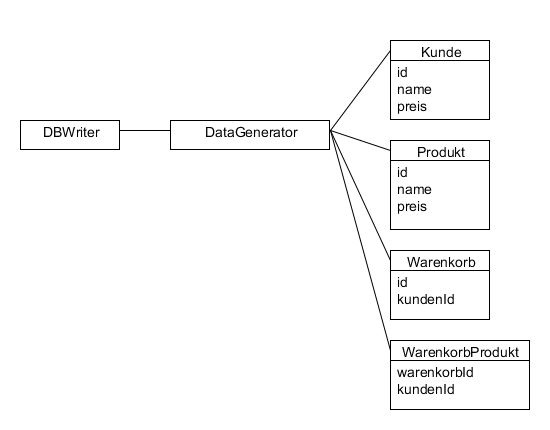
\includegraphics[width=0.8\textwidth]{Ingo/Bilder/AnalyseDatengenerator.png}
\caption{Analyse Datengenerator}
\label{fig:AnalyseDatengenerator}
\end{figure}

\begin{figure}[htp]
\centering
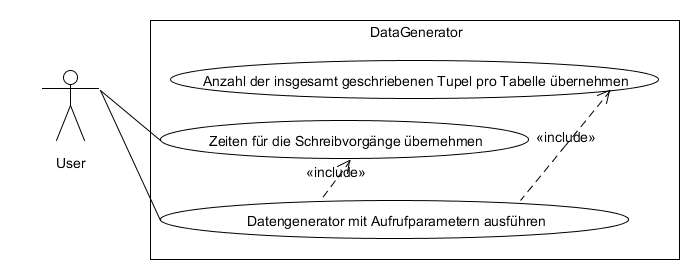
\includegraphics[width=0.8\textwidth]{Ingo/Bilder/AnwendungsfalldiagrammDatengenerator.png}
\caption{Anwendungsfalldiagramm Datengenerator}
\label{fig:AnwendungsfalldiagrammDatengenerator}
\end{figure}


\begin{figure}[htp]
\centering
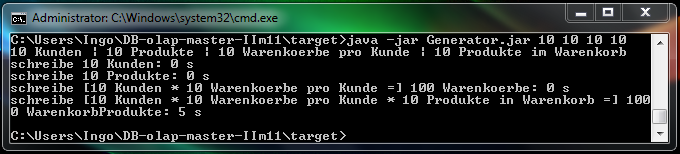
\includegraphics[width=0.8\textwidth]{Ingo/Bilder/UIMockUp.png}
\caption{UI-MockUp}
\label{fig:UI-MockUp}
\end{figure}
\section{Entwurf}
\subsection{Komponentendiagramm}
Abbildung \ref{fig:Komponentendiagramm} auf Seite \pageref{fig:Komponentendiagramm} zeigt das Komponentendiagramm.

\begin{figure}[htp]
\centering
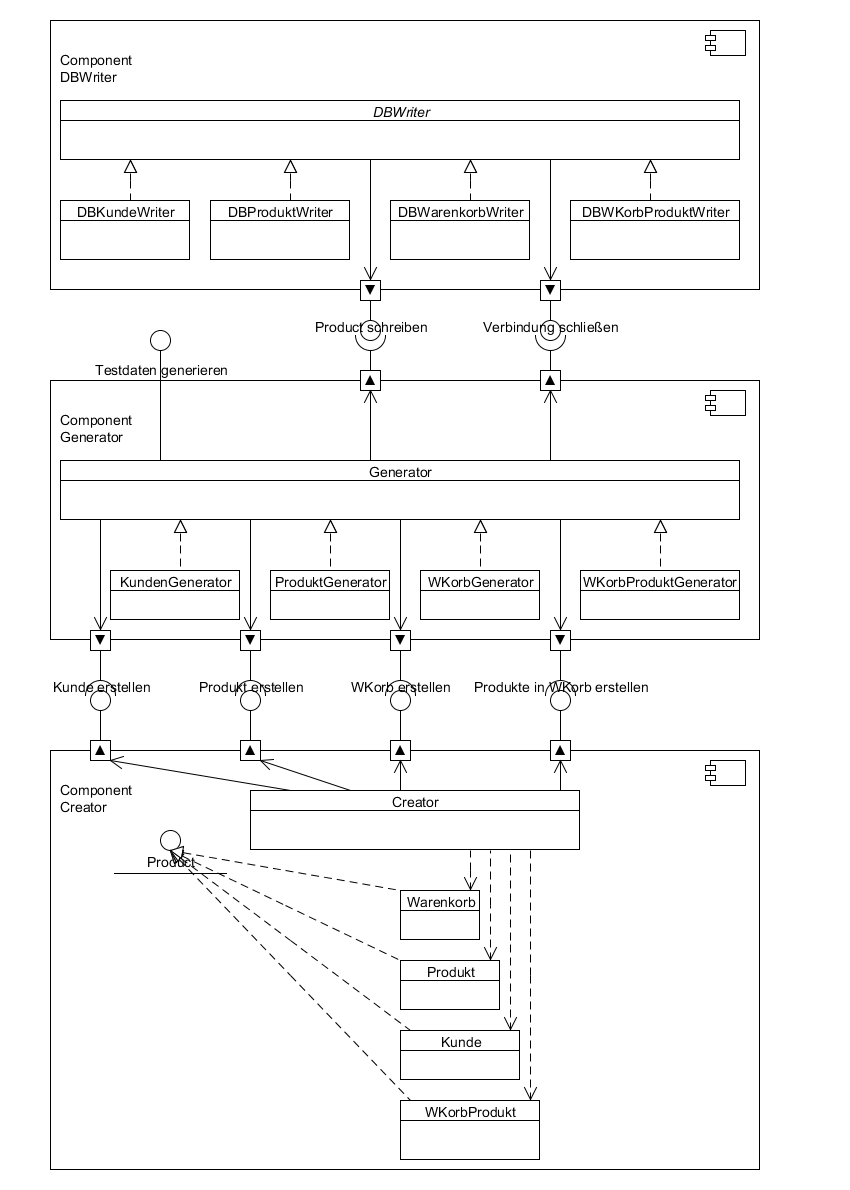
\includegraphics[width=0.8\textwidth]{Ingo/Bilder/Komponentendiagramm.png}
\caption{Komponentendiagramm}
\label{fig:Komponentendiagramm}
\end{figure}

\subsection{Entwurfsklassendiagramm der Generatorkomponente}
Abbildung \ref{fig:EntwurfGeneratorkomponente} auf Seite \pageref{fig:EntwurfGeneratorkomponente} zeigt das Entwurfsklassendiagramm der Generatorkomponente.

\begin{figure}[htp]
\centering
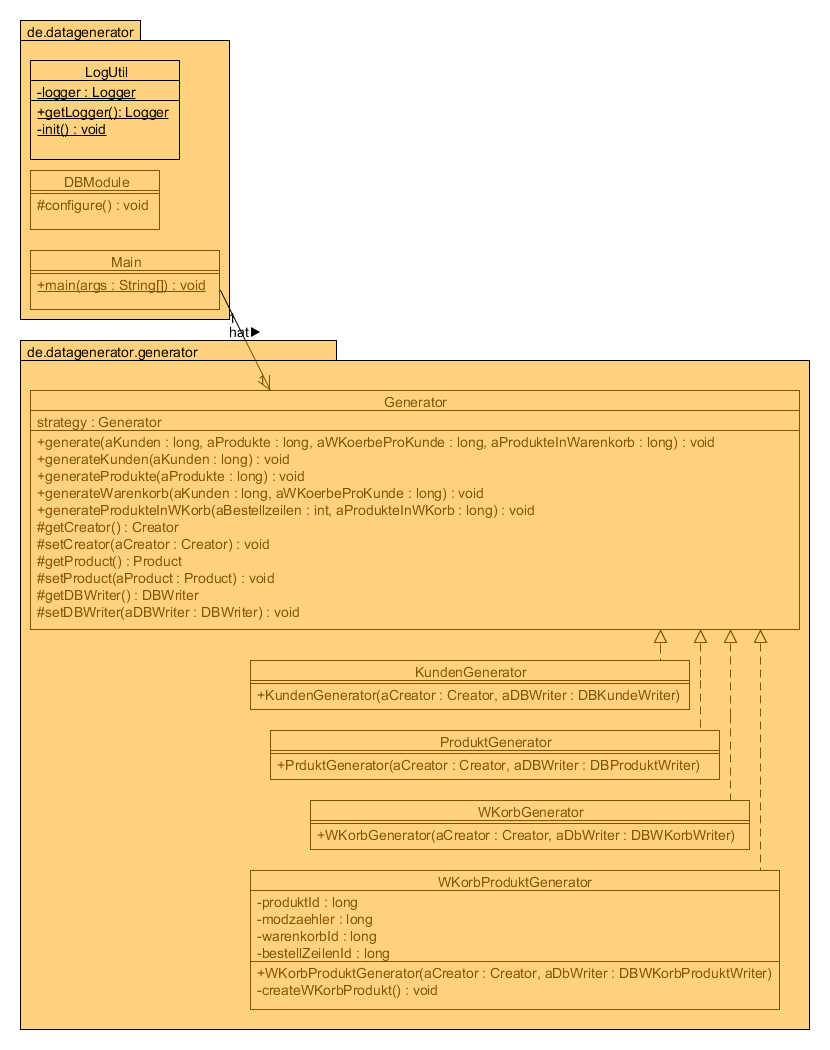
\includegraphics[width=0.8\textwidth]{Ingo/Bilder/EntwurfGeneratorkomponente.png}
\caption{Entwurf der Generatorkomponente}
\label{fig:EntwurfGeneratorkomponente}
\end{figure}

\subsection{Entwurfsklassendiagramm der DBWriterkomponente}
Abbildung \ref{fig:EntwurfDBWriterkomponente} auf Seite \pageref{fig:EntwurfDBWriterkomponente} zeigt das Entwurfsklassendiagramm der DBWriterkomponente.

\begin{figure}[htp]
\centering
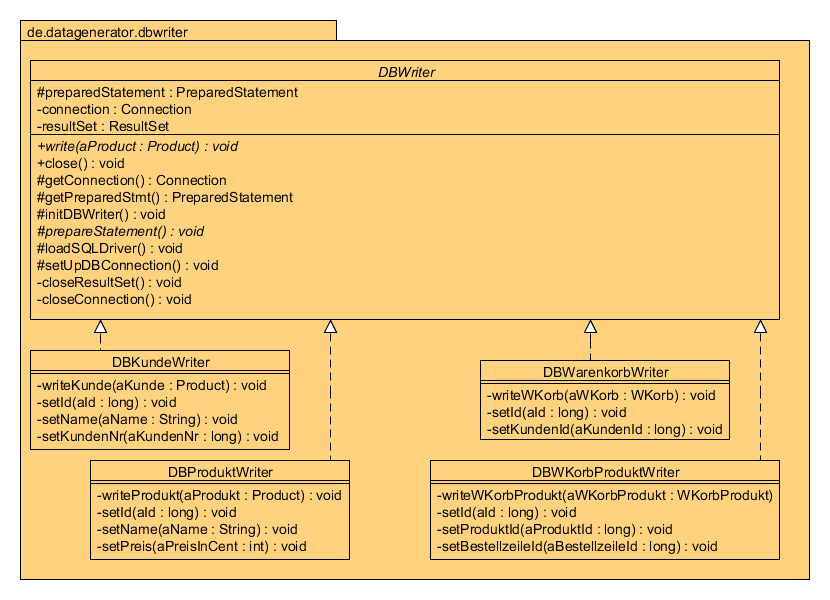
\includegraphics[width=0.8\textwidth]{Ingo/Bilder/EntwurfDBWriterkomponente.png}
\caption{Entwurf der DBWriterkomponente}
\label{fig:EntwurfDBWriterkomponente}
\end{figure}

\subsection{Entwurfsklassendiagramm der Creatorkomponente samt Datamodel}
Abbildung \ref{fig:EntwurfCreatorUndDatamodelKomponente} auf Seite \pageref{fig:EntwurfCreatorUndDatamodelKomponente} zeigt das Entwurfsklassendiagramm der Creatorkomponente und dem dazugeh�rigen Datamodel.

\begin{figure}[htp]
\centering
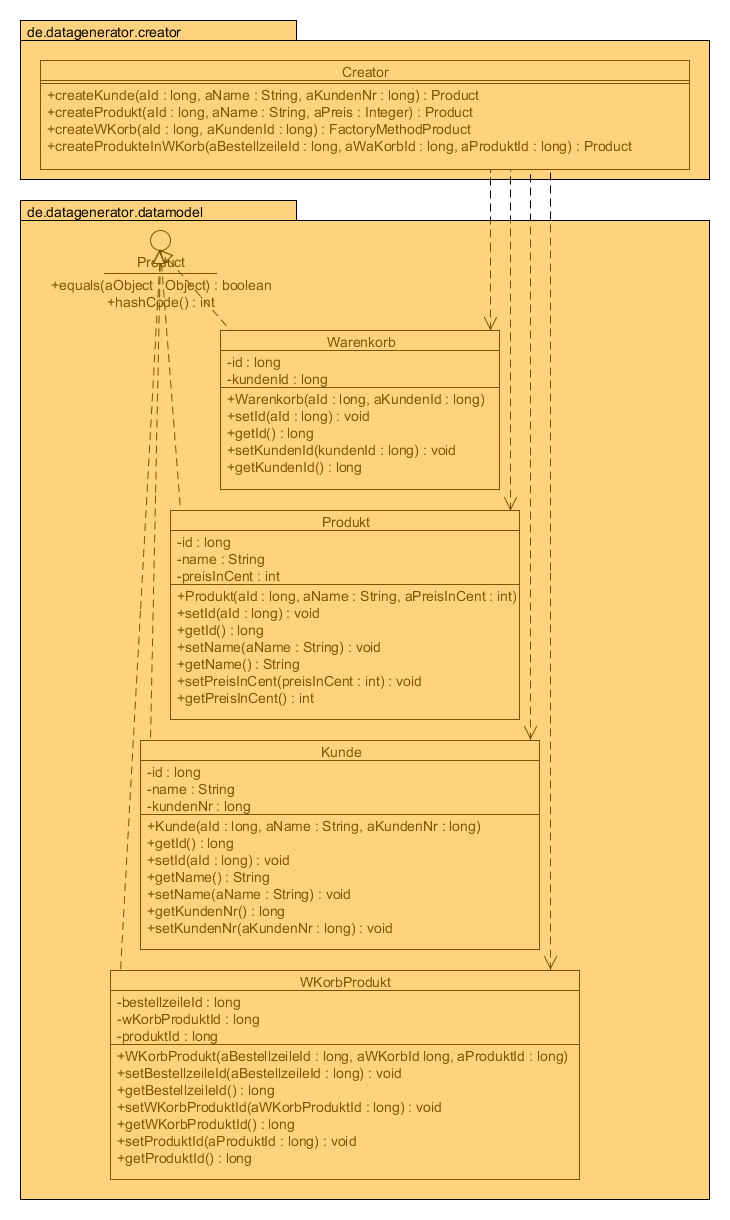
\includegraphics[width=0.8\textwidth]{Ingo/Bilder/EntwurfCreatorUndDatamodelKomponente.png}
\caption{Entwurf der Creatorkomponente}
\label{fig:EntwurfCreatorUndDatamodelKomponente}
\end{figure}

\subsection{Stored Procedures}
Der Generator hat eine zweischichtige Architektur (two tier architecture). Die Komponente Generator greift auf die Dienste der Komponente DBWriter zu. Auch sonst wurde in der Anwendung auf geringe Kopplung geachtet (demeters law).

\subsection{Prepared Statement}
Die generierten Testdaten werden �ber sogenannte Prepared Statements in die Tabellen geschrieben. Prepared Statements enthalten Platzhalter f�r die eigentlich zu schreibenden Daten. Prepared Statements bieten sich u.a. dann an, wenn sich bei dem Statement nur die Parameterwerte unterscheiden. Prepared Statements bringen einen Geschwindigkeitsvorteil, da sie bereits im DBMS vor�bersetzt werden und der DBWriter mit sehr viel generierten Parameterwerten aufgerufen wird.

\subsection{Entwurfsmuster}
Der Creator ist als einfache Fabrik implementiert. Durch ihn werden konkrete Instanziierungen aus dem Clientcode entfernt und somit die Clients von konkreten Klassen entkoppelt (Dependency Inversion Principle)

In z.B. DBWriter konnte initDBWriter() als Template Method implementiert werden. Sie definiert die Schritte f�r die Initialisierung eines DBWriters, wobei die Unterklassen entscheiden, wie sie die abstrakte Hook-Methode prepareStatement() implementieren. Durch die Template Method werden die Highlevel Komponenten loadSQLDriver() und setUpDBConnection() von Lowlevel Komponente prepareStatement() entkoppelt. Die Lowlevel-Komponenten prepareStatement() kann sich in ein System reinh�ngen, und Highlevel Komponenten bestimmen, wann und wie sie erforderlich sind. Die Lowlevel Komponente prepareStatement() ruft Highlevel Komponente nie direkt auf (Hollywood Prinzip).

\subsection{Implementierung und Test}
Das Projekt liegt als Maven-Eclipse-Projekt unter git@github.com:rinkdotrink/DB-olap-master-IIm11.git

\subsubsection{Projektumgebung}
Eclipse-IDE 3.7, JDK 1.7, JUnit 4.8.2, Maven 3, Guice 3, EasyMock 3.0, Log4J 1.2.16, mysql-connector-java 5.1.6, Umlet 11.3

\subsubsection{Projekt aus dem repository laden}
Berechtigungen
git pull

\subsubsection{Maven}

\subsubsection{Maven-Projekt in Eclipse importieren}



\subsubsection{Maven Projekt ausf�hren}
Entweder �ber Jar oder �ber Eclipse

\subsubsection{Jar mit allen Abh�ngigkeiten erstellen}
package


\subsection{Implementierung der Funktionalit�t}
Die drei Komponenten

\subsection{Unit Test mit EasyMock 3.0}
\chapter{MySQL-Datenbank}\label{MySQL-Datenbank}
\section{Die MySQL-Datenbank}

\subsection{MySQL-Architektur}
Die MySQL-Architektur unterscheidet sich deutlich von den Architekturen anderer Datenbanken. Die wichtigste Eigenschaft der MySQL-Datenbank ist die Speichermaschinen-Architekur (engl.: storage-engine architecture), die den Serverprozess mit dem SQL-Parsing und weiteren Funktionalit�ten von der Datenspeicherung und dem Datenabruf entkoppelt. Dabei werden die Tabellen mit den Datens�tzen in speziellen Dateien abgelegt, auf die ausschlie�lich die Speichermaschinen(engl.: storage-engines) Zugriff haben.  Je nach Anforderung und Funktionalit�t der jeweiligen Speichermaschine wird der Zugriff entsprechend organisiert und optimiert.  Die Speichermaschinen-Architektur ist somit der gr��te und gleichzeitig wichtigste Unterschied zu vielen anderen kommerziellen Datenbanken wie z.B. Oracle DB oder DB2. 

\subsection{Der logische Aufbau der MySQL-Architektur}
\begin{enumerate}
 \item Der obersten Schicht sind Dienstprogramme zugeordnet, welche nicht nur von MySQL  ben�tigt werden. Dazu geh�ren Managementdienste und Werkzeuge zur Serververwaltung, die beispielsweise f�r die Behandlung von Verbindungen, Sicherheit, Authentifizierung ben�tigt werden.
 \item Die mittlere Schicht beinhaltet die Hauptfunktionalit�ten der MySQL-Datenbank. Dazu geh�rt Parsing, Optimierung, Analyse und das Caching von Queries. Au�erdem enth�lt sie jegliche Funktionalit�t, die �ber den Speichermaschinen hinweg bereitgestellt wird, wie beispielsweise die Stored Procedures, Trigger und Views.
 \item Die unterste Schicht enth�lt die austauschbaren Speichermaschinen, die jeweils einen unterschiedlichen Tabellentyp verwalten. Die Speichermaschinen sind verantwortlich f�r die Speicherung und den Abruf aller Daten in der MySQL-Datenbank. Jeder Tabellentyp besitzt seine Vor- und Nachteile und ist je nach Anwendungsfall besser oder schlechter geeignet. Der Datenbank-Administrator hat die M�glichkeit den Tabellentyp, in dem die Records gespeichert werden festzulegen und sogar unterschiedliche Tabellentypen in derselben Datenbank zu verwenden.
\end{enumerate}

Die Kommunikation mit dem Server (zwischen der zweiten und der dritten Schicht) basiert auf der Storage-Engine-API. Diese Schnittstelle verdeckt die Unterschiede zwischen den Speichermaschinen und macht sie transparent auf der Query-Ebene. Jede Speichermaschine ist eine Klasse, dessen Instanz mit dem MySQL-Server �ber ein spezielles Handler-Interface kommuniziert. Jeder Thread, der mit einer bestimmten Tabelle arbeiten muss, legt einen Handler an. Der MySQL-Server erteilt dem Handler Befehle,  die solche Operationen wie "`eine Transaktion beginnen"' oder "`Zeile mit dem Prim�rschl�ssel einlesen"' ausf�hren. Die Storage-Engines reagieren auf diese Befehle, die Anfragen aus den h�heren Schichten ausf�hren sollen.

\subsection{Ablauf einer SQL-Abfrage in MySQL}
\begin{enumerate}
 \item Der Client sendet eine Anfrage an den MySQL-Server und noch bevor der Query geparst wird, pr�ft MySQL ob dieser Query nicht schon im Query Cache vorhanden ist.  Falls ein passendes Query gefunden wurde, werden die Zugriffsrechte gepr�ft und die gespeicherten Ergebnisse der Anfrage an den Client gesendet. Ansonsten durchgeht das SQL-Query einen festen Ablaufplan.
 \item Zuerst wird es geparst um Token und einen Parse-Baum zu erhalten.  Mit einem Preprozessor wird untersucht ob alle Tabellen und Spalten aus der Abfrage existieren, au�erdem werden jegliche Namen aufgel�st und Zugriffsrechte gepr�ft. Anschlie�end werden mit einer Query Optimierung  unn�tige Dateizugriffe minimiert und es wird nach einer m�glichst schnellen Anfragebearbeitung gesucht. Der Query-Optimizer erstellt einen sogenannten Ausf�hrungsplan (engl.: execution plan).
 \item Die Abfrageausf�hrungs-Engine (engl.: query execution engine) f�hrt Schritt f�r Schritt den Ausf�hrungsplan aus und  ruft dabei die API-Befehle der entsprechenden Engine auf.
 \item Zum Schluss wird das Abfrage-Ergebnis an den Client gesendet. Wenn der Query cacheable ist, wird das Ergebnis der Abfrage im Query Cache gespeichert.
\end{enumerate}

\begin{figure}[htp]
\centering
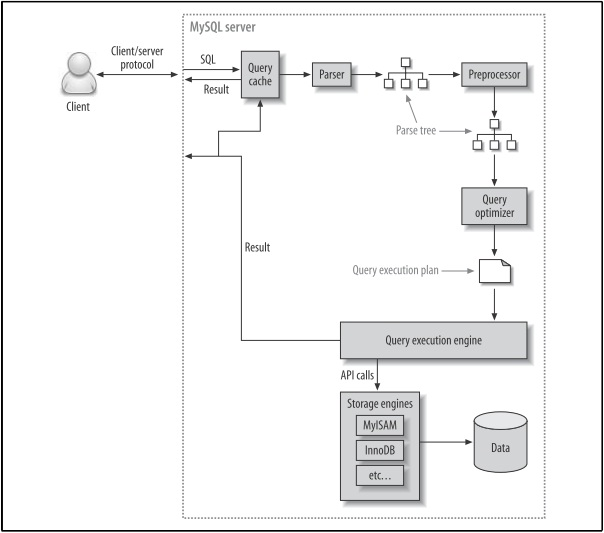
\includegraphics[width=0.75\textwidth]{Christof/Bilder/QueryEx.jpg}
\caption{Query-Ausf�hrungspfad}
\label{fig:QueryEx}
\end{figure}

\subsection{Speichermaschinen und Tabellentypen}\label{Speichermaschinen}
Es stellt sich nun die Frage, wodurch sich die verschiedenen Tabellentypen voneinander unterscheiden und  nach welchen Kriterien w�hlt man die richtige Storage-Engine aus. 
Grunds�tzlich lassen sich die Tabellentypen in transaktionssichere und nicht-transaktionssichere einteilen, die jeweils unterschiedliche Vorteile haben.

Transaktionssichere Tabellen sind ACID-konform und haben den Vorteil, dass man bei einem Systemabsturz oder bei  Hardwareausf�llen die Daten auf jeden Fall mit Hilfe der automatischen Wiederherstellung oder der Sicherungskopie und dem Transaktionslog zur�ckbekommt. Wenn Autocommit deaktiviert wurde, k�nnen mehrere Anweisungen zusammengefasst und auch �nderungen mit einem ROLLBACK verworfen werden. Wenn ein Update fehlschl�gt, werden alle �nderungen im Gegensatz zu nichttransaktionssicheren Tabellen r�ckg�ngig gemacht. 

Der wichtigste Vorteil von nichttransaktionssichere Tabellen ist die Geschwindigkeit un der Speicherverbrauch im RAM und auf der Festplatte.


\subsubsection{MyISAM-Engine}
Sie verwaltet nichttransaktionssichere Tabellen. Unter anderem bietet sie eine Volltextindizierung und Komprimierung an. Es werden jedoch nur die Indexbl�cke im Cache(Key Buffer) zwischengespeichert, und f�r die einzelnen Datens�tze wird der Dateisystem-Cache des Betriebssystems(Operating system cache) benutzt.  Aus diesem Grund macht es Sinn dem Dateisystem-Cache mehr Speicher zur Verf�gung zu stellen als dem Key Buffer. Bei MyISAM wird jede Tabelle in drei Dateien auf der Festplatte gespeichert:  das Tabellenformat(Tabellenname.frm), die Datendatei(Tabellenname.MYD) und die Indexdatei(Tabellenname.MYI).  Bei einem Datanbank-Lock wird die komplette Tabelle gesperrt, was unter Umst�nden einen Flaschenhals darstellen kann. Um mehr Geschwindigkeit zu erzielen, ist es empfehlenswert mit entsprechenden Tabellenoptionen die Daten- und Indexdatei in unterschiedliche Verzeichnisse zu legen. 

\subsubsection{InnoDB-Engine}
Sie ist die Standard-Storage-Engine und verwaltet transaktionssichere Tabellen. Es werden die vier Isolationslevel(Read Uncommited, Read Commited, Repeatable Read und Serializalbe)implementiert und mithilfe von Multiversion Concurrency Control wird eine sehr hohe Parallelit�t erreicht.  Die Daten werden in einer oder mehreren Datendateien abgespeichert, die zusammen als ein Tablespace bezeichnet werden. Der Tablespace wird vollst�ndig von der InnoDB-Engine verwaltet. Es sind somit im Gegensatz zu MyISAM Tabellen beliebiger Gr��e m�glich. Ein weiteres wichtiges Merkmal von der Inno-DB-Engine ist, dass bei einem Datenbank-Lock nur die jeweilige Zeile gesperrt wird und bei SELECT-Anweisungen konsistente Leseoperationen ohne Sperren m�glich sind. Au�erdem werden sowohl die Indizes als auch die Daten im eigenen Bufferpool zwischengespeichert.

\subsubsection{Memory}
Sie bietet eine nicht-transaktionssichere Verwaltung von Tabellen im Arbeitsspeicher an. Die Daten sind somit nicht permanent gesichert. Diese Daten-Engine unterst�tzt auch nicht die Option AUTO\_INCREMENT und die Datentypen BLOB oder TEXT. Diese Speicher-Engine eignet sich vor allem f�r einen sehr schnellen Datenzugriff.

\subsubsection{Archive}
Mit der Speicher-Engine Archive k�nnen gro�e Datenmengen ohne Indizes mit einem sehr kleinen Speicherverbrauch verwaltet werden. Die Zeilen werden bei einer INSERT-Anweisung komprimiert und im Kompressionspuffer gespeichert.  Es werden INSERTs und SELECTs unterst�tzt, nicht jedoch DELETE, REPLACE oder UPDATE. Archive nutzt genauso wie die InnoDB Zeilensperren.
\section{Optimierungsma�nahmen}\label{Optimierungsmassnahmen}

\subsection{Indizes}\label{Indizes}
Ein Index ist bei der MyISAM eine zus�tzliche Datei und bei der InnoDB ein zus�tzlicher Dateibereich mit sortierten Querverweisen auf die Datens�tze einer Tabelle, was unter Umst�nden bei Suchvorg�ngen enorme Geschwindigkeitsvorteile mit sich bringt. Ohne eine Indizierung m�sste die Datenbank die Suche bei dem ersten Datensatz beginnen und dann die gesamte Tabelle sequentiell nach passenden Datens�tzen durchforsten. Mit einem Index kann die Suche an einer bestimmten Position in der Mitte der Datendatei beginnen, was eine gezielte und schnelle Suche erm�glicht.
Indizes eignen sich nur f�r Spalten, nach denen oft gesucht wird oder die man sortieren m�chte. Bei Datens�tzen, die oft ver�ndert werden, sind Indizes nicht geeignet, da bei jeder �nderung auch der Index ver�ndert werden muss. Bei den InnoDB-Tabellen werden die Indizes auch zum Row-Level-Locking verwendet, um die gesperrten Datens�tze intern zu kennzeichnen, was aus Performancegr�nden im Index erfolgt und nicht in den eigentlichen Tabellen. MySQL unterst�tzt die B-Tree-Indizierung sowie die Hash-Indizierung. 

\subsubsection{B-Tree-Indizierung}
Ein B-Tree-Index eignet sich gut f�r Ausdr�cke mit Vergleichsoperatoren und beim dem BETWEEN-Operator. Auch ein LIKE-Vergleich ist m�glich wenn das Argument ein Konstanten-String ist, der nicht mit einem Jokerzeichen(=\%) beginnt.  Ein B-Tree-Index eignet sich auch f�r das Sortieren oder Gruppieren einer Tabelle.
MySQL kann auch mehrspaltige Indizes erstellen, dabei muss man jedoch beachten,  dass bei den Abfragen immer die erste Spalte des Indexes in einer WHERE-Klausel angegeben wird, sonst wird der Teil-Index nicht benutzt:
\begin{verbatim}
	z.B. INDEX name(nachname,vorname)
	
	Index wird benutzt 				-> SELECT *FROM test WHERE nachname="'Schmidt"'
	Index wird nicht benutzt  -> SELECT *FROM test WHERE vorname ="'Hans"'
\end{verbatim}
Das bedeutet, dass wenn beispielsweise ein dreispaltiger Index f�r (Spalte1,Spalte2,Spalte3) angelegt wird, wird er f�r (Spalte1),(Spalte1,Spalte2) und (Spalte1,Spalte2,Spalte3) eingesetzt. F�r (Spalte2) und f�r (Spalte2,Spalte3) kommt die Suchfunktionalit�t mit dem Index nicht zum Einsatz. Das muss man bei der Erstellung von SQL-Anweisungen beachten.
Au�erdem muss der Index alle AND-Ebenen in der WHERE-Klausel einbeziehen, sonst wird er ebenfalls nicht zur Optimierung benutzt:
\begin{verbatim}
	z.B. INDEX anschrift(nachname,vorname,ort)
	
	wird benutzt			  -> WHERE nachmame = "`Schmidt"' AND 
														vorname = "`Hans"' AND ort"'Halle"'	
	wird nicht benutzt  -> WHERE vorname ="'Hans"' AND ort ="'Buxtehude"'
\end{verbatim}
Wenn eine Abfrage auf einen gro�en Anteil von Datens�tzen zugreifen muss, kann es passieren, dass der Optimierer auf die Verwendung eines Indexes verzichtet und einen Full Table-Scan anordnet, da dadurch sich weniger Suchvorg�nge ergeben. Wenn aber die Abfrage eine LIMIT-Klausel enth�lt, und somit nur ein paar Datens�tze abgerufen werden sollen, wird trotzdem ein Index verwendet, da sich diese Datens�tze mit dem Index schneller finden lassen.
\subsubsection{Hash-Indizierung}
Ein Hash-Index unterscheidet sich grunds�tzlich dadurch, dass er nur vollst�ndige Schl�ssel zur Suche nach einem Datensatz verwenden kann. Au�erdem kann der Optimierer einen Hash-Index nicht zur Beschleunigung von ORDER-BY-Operationen verwenden und auch f�r Vergleiche mit  \textbf{\tt< \tt>} ist er nicht geeignet. Der Hash-Index eignet sich aber sehr gut f�r Vergleiche mit den Operatoren = oder \textbf{\tt< = \tt>}

\subsection{Partitionierung}\label{Partitionierung}
Bei der Partitionierung werden die Daten der einzelnen Tabellen nach bestimmten Regeln getrennt und auf mehrere physikalische Einheiten verteilt. Die Regel wird von dem Benutzer ausgew�hlt und als Partitionierungsfunktion bezeichnet. Es kann sich dabei um Modulus, um eine Hash-Funktion oder um einen Vergleich mit einer Menge von Wertebereichen oder Wertelisten handeln.
MySQL unterst�tzt nur die horizontale Partitionierung. Dabei werden die Tabellen zeilenweise getrennt. 

\subsubsection{Partitionierungsfunktionen in MySQL}
\begin{enumerate}
\item \textbf{Range Partitioning} \\
Den verschiedenen Partitionen werden Zeilen zugeordnet, deren Spaltenwerte einem bestimmten Wertebereich entsprechen. Beispielsweise die verkauften Produkte im ersten Quartal w�re eine Partition und die verkauften Produkte im zweiten Quartal w�re eine weitere Partition.

\item \textbf{List Partitioning} \\
Diese Methode ist dem Range Partitioning �hnlich. Der Unterschied ist nur der, dass die Kriterien nicht fortlaufend sein m�ssen und willk�rlich ausgew�hlt werden k�nnen. Es wird eine Entscheidungsliste f�r jede Partition erstellt. Beispielsweise die verkauften Produkte in den Jahren 02, 04, 06 w�re eine Partition und eine weitere Partition w�ren die verkauften Produkte in den Jahren 01, 03, 05.

\item \textbf{Hash Partitioning und Linear Hash-Partitioning} \\
Bei dieser Methode werden die Daten gleichm��ig verteilt. F�r den Hash gibt man haupts�chlich einen Spaltenwert an. Meistens wird dabei die Modulo-Funktion verwendet und bei dem linearen Hashing ein linearer Zweierpotenz-Algorithmus. 

\item \textbf{Key Partitioning} \\
Diese Partitionierung ist der  Hash-Partitionierung sehr �hnlich. Der Unterschied besteht darin, dass der Prim�rschl�ssel der Tabelle als Kriterium dient und dieser wird f�r die MD5-Operation verwendet.

\item \textbf{Subpartitioning} \\
Es besteht die M�glichkeit die partitionierten Tabellen noch weiter zu unterteilen.

\end{enumerate}

\chapter{Performancetest}\label{Performancetest}
\section{Testvorbereitung}\label{Testvorbereitung}
Wir w�hlen die InnoDB als Speichermaschine aus, da sie die Transaktionssicherheit gew�hrleistet und sich dadurch f�r das Betreiben eines Webshops am besten eignet. 
Jede Versuchsreihe entspricht einer bestimmten Konfiguration und besteht aus vier Testl�ufen zu je einem Use Case. Am Anfang  werden Testdaten mit einer  bestimmten Anzahl von Kunden, einer konstanten Anzahl von Produkten (1000), einer konstanten Anzahl von Warenk�rben pro Kunde(5) und genauso einer konstanten Anzahl von Produkten pro Warenkorb(5) generiert. Die Anzahl der Kunden erh�ht sich mit jedem Testlauf. In jeder Versuchsreihe werden die vier verschiedenen Use Cases betrachtet, die durch eine unterschiedliche SELECT-Anweisung an die MySQL-Datenbank realisiert werden:
\subsection{SELECT-Anweisungen}\label{Select}
\begin{enumerate}
\item \textbf{Use Case 1: Welches Produkt wurde wie oft gekauft?}
\lstset{language=Java,caption={UseCase1},label=Use Case 1}
\lstinputlisting[language=Java]{Christof/Listings/UseCase1.java}
\item \textbf{Wie viel Umsatz wurde von wem in einem bestimmtem Zeitraum generiert?}
\lstset{language=Java,caption={UseCase2},label=Use Case 2}
\lstinputlisting[language=Java]{Christof/Listings/UseCase2.java}
\item \textbf{Wie viele Kunden haben an einem bestimmten Zeitpunkt bestellt?}
\lstset{language=Java,caption={UseCase3},label=Use Case 3}
\lstinputlisting[language=Java]{Christof/Listings/UseCase3.java}
\item \textbf{Wer hat wieviel an den gegebenen neun Tagen umgesetzt?}
\lstset{language=Java,caption={UseCase4},label=Use Case 4}
\lstinputlisting[language=Java]{Christof/Listings/UseCase4.java}
\end{enumerate}


\subsection{EXPLAIN-Anweisung}\label{ExplainAnweisung}
Bei den SQL-Abfragen stellten wir bei jeder SELECT-Anweisung ein EXPLAIN davor, um n�tzliche Informationen zum Ausf�hrungsplan des Optimierers zu erhalten. Die EXPLAIN-Anweisung liefert u.a. Daten dar�ber, ob die Indizes auch wirklich benutzt wurden, in welcher Reihenfolge die Tabellen verkn�pft werden sowie weitere Informationen, die helfen sollen die SELECT-Anweisungen zu beschleunigen.
\subsubsection{Beispiel 1}
\begin{figure}[htp]
\centering
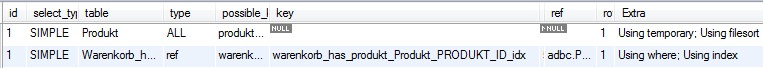
\includegraphics[width=1\textwidth]{Christof/Bilder/ExplainB1.jpg}
\caption{Explain-Tabelle1}
\label{fig:explain1}
\end{figure}
An diesem Beispiel sieht man das Ergebnis einer EXPLAIN-Anweisung. Das \textit{ALL} bei \textbf{type} besagt, dass zuerst alle Datens�tze aus der Produkt-Tabelle gelesen werden. Das \textit{Using temporary} bedeutet, dass sogar eine tempor�re Tabelle erzeugt wird, um Zwischenergebnisse zu speichern. In der Spalte \textbf{key} sieht man, dass sich der Optimierer f�r den Index \textbf{warenkorb\_has\_produkt\_Produkt\_PRODUKT\_ID\_idx} entschieden hat. Mit Zuhilfenahme dieses Indexes wird die Verbindung zu der Tabelle \textbf{warenkorb\_has\_prdukt} geschaffen.
\subsubsection{Beispiel 2}
\begin{figure}[htp]
\centering
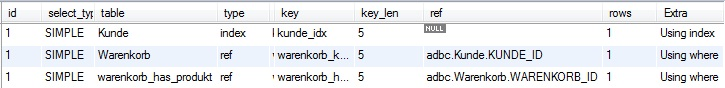
\includegraphics[width=1\textwidth]{Christof/Bilder/ExplainB2.jpg}
\caption{Explain-Tabelle2}
\label{fig:explain2}
\end{figure}
In der Spalte \textit{Extra} bedeutet der Kommentar \textbf{Using index}, dass MySQL das Ergebnis der Abfrage komplett aus dem Index erstellen kann und dabei keine Daten aus der Tabelle nimmt. In der Spalte \textit{type} k�nnen folgende Werte vorkommen(angefangen mit dem schlechtesten):
\begin{itemize}
\item \textbf{all}: Es wird kein Index benutzt weil er nicht besteht oder nicht brauchbar ist.
\item \textbf{index}: Der gesamte Index wird �berpr�ft.
\item \textbf{range}: Alle Datens�tze in einem bestimmten Bereich werden aus der Tabelle gelesen. Die Datens�tze werden anhand eines Indexes ausgew�hlt.
\item \textbf{ref}: Alle Datens�tze mit passenden Indexwerten werden aus der Tabelle gelesen. Wird verwendet bei nicht eindeutigen Schl�sseln, oder f�r indizierte Spalten die mit Hilfe der Operatoren = oder \textbf{\tt < = \tt>} verglichen werden.
\item \textbf{eq\_ref}: F�r jede einzelne Zeile aus der Tabelle1 wird eine Zeile aus der Tabelle2 gelesen. Kann verwendet werden f�r indizierte Spalten, die mit Hilfe des Operators = verglichen werden.
\end{itemize} 
  
\subsection{EXPLAIN PARTITIONS-Anweisung}\label{ExplainPartitions}
Diese Anweisung liefert zus�tzlich Informationen �ber die verwendeten Partitionen. Man kann sie jedoch nur auf RANGE- oder LIST-partitionierte Tabellen verwenden. Bei KEY- oder HASH-Partitionen ist sie unbrauchbar, da automatisch alle Partitionen ausgegeben werden.

\subsection{Konfigurationen der MySQL-Datenbank und der Tabellen}\label{Konfiguration}
Jede Versuchsreihe testet die SELECT-Anweisungen mit einer bestimmten Konfiguration der MySQL-Datenbank und der Tabellen. Vor jedem Testlauf werden die entsprechenden Konfigurationseintellungen mit SQL-Anweisungen durchgef�hrt.
\begin{enumerate}
\item \textbf{K1} : Kaltstart ohne Index
\item \textbf{K2} : Kaltstart ohne Index
\item \textbf{K3} : Hash-Indizes auf Primary Keys und Foreign Keys / ohne Partitioning
\item \textbf{K4} : B-Tree-Indizes auf Primary Keys und Foreign Keys / ohne Partitioning
\item \textbf{K5} : Hash-Indizes auf Primary Keys und Foreign Keys sowie B-Tree-Index auf Datum / ohne Partitioning
\item \textbf{K6} : Hash-Indizes auf Primary Keys und Foreign Keys sowie B-Tree-Index auf Datum / mit List-Partitioning auf MONTH(Datum) f�r jedes Quartal
\item \textbf{K7} : Hash-Indizes auf Primary Keys und Foreign Keys sowie B-Tree-Index auf Datum / mit Hash-Partitioning auf MONTH(Datum) f�r jeden Monat
\item \textbf{K8} : Hash-Indizes auf Primary Keys und Foreign Keys sowie B-Tree Index auf Datum / mit Range-Partitioning auf COLUMNS(Datum) f�r jedes Quartal
\item \textbf{K9} : Hash Indizes auf Primary Keys und Foreign Keys sowie B-Tree-Index auf Datum / mit Sub-Partitioning (Range-Partitioning quartalsweise auf Datum und f�r jedes Quartal jeweils vier Hash-Partitions auf TO\_DAYS(Datum))
\item \textbf{K10}: Hash-Indizes auf Primary Keys und Foreign Keys / mit Sub-Partitioning (Range-Partitioning quartalsweise auf Datum und f�r jedes Quartal jeweils vier Hash-Partitions auf TO\_DAYS(Datum)
\end{enumerate} 

\section{Testdurchf�hrung}\label{Testdurchfuehrung}

\subsection{Annahmen und Vor�berlegungen}\label{Annahme}
\begin{enumerate}
\item \textbf{K1 und K2} \\ 
Zuerst wurde zweimal ein Kaltstart ohne Index(\textbf{K2}) durchgef�hrt, um Referenzwerte zu bekommen, bevor die Testl�ufe mit der Indizierung und Partitionierung begonnen werden. Alle nachfolgenden Messungen wurden ebenfalls mit einem deaktivierten Query-Cache durchgef�hrt, damit die Messwerte, die abh�ngig von der Gr��e der Kundentabelle sind, durch das Zwischenspeichern nicht verf�lscht werden. 
\item \textbf{K3 und K4} \\
Das Hinzuf�gen von Indizes ist der erste wichtige Schritt bei der Optimierung von SELECT-Anweisungen und sollte bei der richtigen Formulierung der SELECT-Anweisung einen enormen Geschwindigkeitsvorteil gegen�ber Abfragen auf Tabellen ohne Indizes bieten. Es ist die Frage zu beantworten, ob es bei den vier Use Cases einen gro�en Geschwindigkeitsunterschied zwischen der Hash-Indizierung(\textbf{K3}) und der B-Tree-Indizierung(\textbf{K4}) gibt und wodurch sich eventuelle Unterschiede ergeben.  
\item \textbf{K5} \\ 
Wenn man die Konfiguration K3 nehmen und diese um ein B-Tree-Index auf das Datum(\textbf{K5}) erg�nzen, sollten bei dem UseCase3 die Zeilen mit dem gesuchten Datum schneller gefunden werden als ohne den B-Tree-Index.
\item \textbf{K6} \\ 
Mit einer zus�tzlichen List-Partitionierung auf die drei Monate in jedem Quartal (\textbf{K6}) m�sste die Suche nach einem konstanten Datumswert, wie es im UseCase3 der Fall ist, beschleunigt werden, denn er m�sste nur in der einen Partition suchen. Interessant ist hierbei auch, wie die List-Partitionierung mit \textbf{BETWEEN} beim UseCase2 umgeht.    
\item \textbf{K7} \\ 
Mit einer Hash-Partitionierung auf die 12 Monate (\textbf{K7}) w�rde es einen Vorteil bringen, wenn nur auf eine bzw. im UseCase4 auf drei Partitionen zugegriffen wird. Wenn jedoch alle Partitionen durchsucht werden, dann bringt es Nachteile. Es stellt sich wieder die Frage, wie reagiert die Hash-Partitionierung auf eine \textbf{BETWEEN}-Anweisung.  
\item \textbf{K8} \\
Die Range-Partitionierung auf die Quartale(\textbf{K8}) sollte eigentlich die Geschwindigkeit f�r den UseCase2 mit der \textbf{BETWEEN}-Anweisung verk�rzen. Denn bei dem verwendeten Range entspricht eine Partition jeweils einem Quartal und im UseCase2 wird die Datum-Spalte nach Werten in einem Quartal durchsucht.
\item \textbf{K9 und K10} \\
Die Konfiguration \textbf{9} unterscheidet sich von der Konfiguration \textbf{10} dadurch, dass sie ein B-Tree-Index auf das Datum enth�lt. Bei beiden Konfigurationen werden insgesamt 16 Teilpartitionen auf das Datum erstellt. Es soll dadurch herausgefunden werden, ob die Teilpartitionierung bei diesen \textbf{SELECT}-Anweisungen die Ausf�hrung beschleunigt. 
\end{enumerate}
\subsection{Testergebnisse bei einer Million Kunden}\label{Testergebnisse}
In der darunterliegenden Tabelle werden die Messergebnisse f�r \textbf{K3} bis \textbf{K10}  bei einer Anzahl von einer Million Kunden dargestellt. Diese Messwerte sind am aussagekr�ftigsten und wurden deshalb f�r die Analyse von den anderen Messwerten hervorgehoben. Alle anderen Messwerte dienten bei der Analyse dazu, um Vergleichswerte zu haben und um eventuelle Messfehler aufzudecken. Alle Messwerte sind Angaben in Sekunden. 
\begin{figure}[htp]
\centering
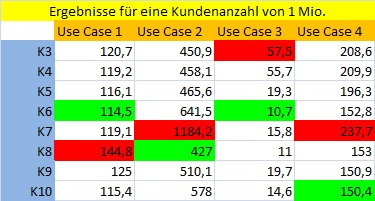
\includegraphics[width=0.75\textwidth]{Christof/Bilder/auswert1.jpg}
\caption{Testergebnisse}
\label{fig:auswert1}
\end{figure}

\subsection{Testauswertung}\label{Testauswertung}
\begin{enumerate}
\item \textbf{K1 und K2} \\ 
Beim Kaltstart ohne Index(\textbf{K1 und K2}) wurden die meisten Testl�ufe abgebrochen, da es l�nger als 20 Minuten gedauert hat. 
\item \textbf{K3 und K4} \\ 
Die Indizes brachten wie erwartet einen enormen Geschwindigkeisunterschied, bei 100 Tausend Kunden hat die Abfrage f�r den UseCase1 um den Faktor 29 k�rzer gedauert. Im direkten Vergleich zwischen \textbf{K3} und \textbf{K4} gab es so gut wie keine Unterschiede bei allen Use Cases. Auch der Ausf�hrungsplan mit Hilfe der \textbf{EXPLAIN}-Anweisung zeigte keine Unterschiede bei den Zugriffstypen. Bei allen Use Cases wurde auf die selbe Art auf die Tabellen zugegriffen.    
\item \textbf{K5} \\ 
Die Vermutung hat sich best�tigt und bei dem UseCase3 gibt es eine deutliche Performancesteigerung um den Faktor 3 mit dem zus�tzlichen B-Tree-Index auf das Datum(\textbf{K5}). Es bleibt nun aber die Frage zu kl�ren, wieso sich der UseCase2 mit der \textbf{K5} als einziger verschlechtert hat, obwohl die Zugriffstypen im Vergleich zur K3 die selben sind, und die B-Tree-Indizierung f�r \textbf{BETWEEN}-Operatoren eigentlich gut geeignet ist. Wenn man sich den Ausf�hrungsplan anschaut, dann erkennt man, dass bei K3 der Optimierer bei der Verkn�pfung der Tabellen zuerst einen vollst�ndigen Tabellenscan mit der Tabelle Kunde durchf�hrt, die 25-Mal kleiner ist als die \textbf{Warenkorb\_Has\_Product} Tabelle. Und bei \textbf{K5} f�ngt er zuerst mit der sehr gro�en Tabelle \textbf{Warenkorb\_Has\_Product} an, was trotz der Indizierung etwas l�nger dauert als wenn er einen vollst�ndigen Tabellenscan mit der Tabelle Kunde gleich zu Beginn der Verkn�pfung durchf�hrt. Wahrscheinlich ist das der Grund wieso der UseCase2 mit \textbf{K6} um 15 sek schlechter ist als mit \textbf{K3}. 
\item \textbf{K6} \\ 
Der UseCase3 ist mit \textbf{K6} tats�chlich noch schneller ausgef�hrt worden, was haupts�chlich an der List-Partitionierung liegt und dadurch nur eine Partition durchsucht wird. Die Zeit f�r den UseCase2 hat sich jedoch bei \textbf{K6} um 190 sek im Vergleich zur K3 verschlechtet. Das liegt wahrscheinlich daran, dass er wieder mit der gro�en Tabelle \textbf{Warenkorb\_Has\_Produkt} beginnt und aufgrund der \textbf{BETWEEN}-Anweisung alle Partitionen durchsucht werden.
\item \textbf{K7} \\  
Der Wert f�r UseCase2 ist bei \textbf{K7} doppelt so schlecht wie bei K6, der Grund daf�r ist wahrscheinlich das Hash-Partitionierung mit der \textbf{BETWEEN}-Anweisung �berhaupt nicht klar kommt. Mit EXPLAIN-Partitions zeigt, dass er auf alle 12 Partitionen zugreift anstatt nur auf 3. Der UseCase4 schneidet bei \textbf{K7} ebenfalls am schlechtesten ab, worauf man bisher noch keine annehmbare Antwort gefunden hat und was noch zu erforschen w�re. 
\item \textbf{K8} \\
Die Range-Partitionierung geht mit der \textbf{BETWEEN}-Anweisung am besten um und wir erhalten somit f�r den UseCase2 mit der \textbf{K8} das beste Ergebnis, weleches um den Faktor 2,77 besser ist als mit der Hash-Partitionierung mit K7. Beim UseCase1 muss er sowieso die ganze Tabelle \textbf{Produkt} durchsuchen und nimmt somit keinen Index auf den Schl�ssel. Die Frage bleibt jedoch noch zu kl�ren wieso der UseCase1 bei der Hash-Partitionierung mit K7 um 25 sek besser abschneidet als mit \textbf{K8}.
\item \textbf{K9 und K10} \\ 
Die Teilpartitionierung mit einem B-Tree-Index auf das Datum liefert bei allen Use Cases ein relativ gutes Ergebnis und erweist sich als die beste Konfiguration bei diesen Anwendungsf�llen. Vor allem bei dem UseCase1 und UseCase4 sind die Messwerte mit \textbf{K9} im Vergleich zu anderen Konfigurationen besonders gut.      
\end{enumerate}

\subsection{Alle Messwerte}\label{Alle}
\begin{figure}[htp]
\centering
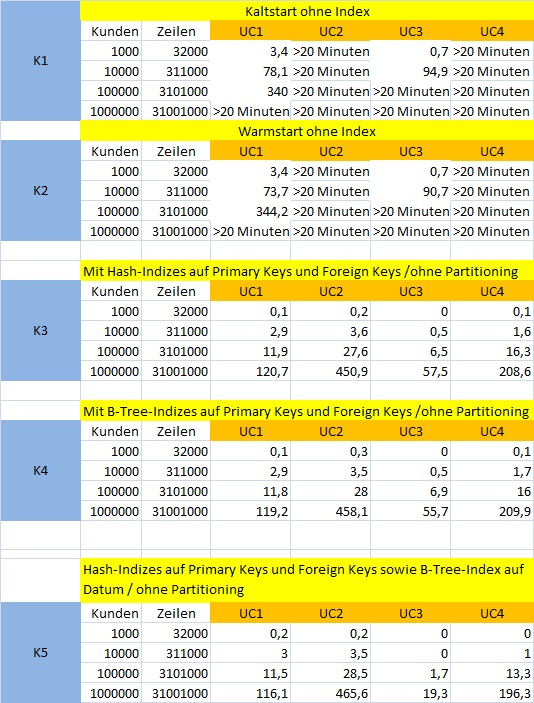
\includegraphics[width=1\textwidth]{Christof/Bilder/TabTeil1.jpg}
\caption{Messwerte Teil 1}
\label{fig:erg1}
\end{figure}

\begin{figure}[htp]
\centering
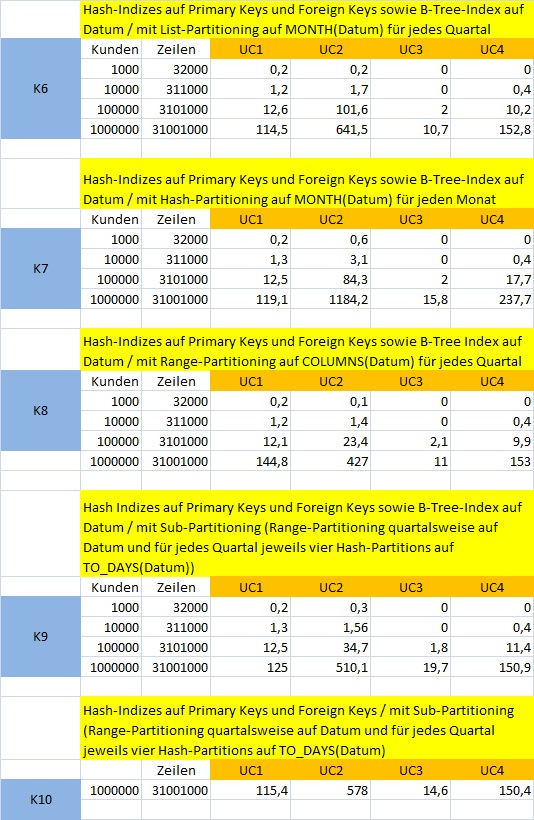
\includegraphics[width=1\textwidth]{Christof/Bilder/TabTeil2.jpg}
\caption{Messwerte Teil 2}
\label{fig:erg2}
\end{figure}



 
\newpage
\section{Zusammenfassung} \label{Summary}
\begin{table}[h]
	\centering
		\begin{tabular}{|c|c|}
		\hline
		K4  & 0,993830822 \\ \hline
		K5  & 1,050671015 \\ \hline
		K6  & 0,911038608 \\ \hline
		K7  & 0,538090956 \\ \hline
		K8  & 1,13848872  \\ \hline
		K9  & 1,039717016 \\ \hline
		K10 & 0,975885368 \\ \hline			
		\end{tabular}
	\caption{Ver�nderung im Vergleich zu K3}
	\label{tab:VergleichZuK3}
\end{table}

In Tabelle \ref{tab:VergleichZuK3} sind die Faktoren abzulesen, um die sich die Abfragen im Durchschnitt verbessern oder verschlechtern. Da Konfiguration 3 (K3) bereits erheblich schneller ist als K1 oder K2 wurde sie dabei als Referenz benutzt. Bei der Analyse der Daten f�llt auf, dass f�r unsere Versuche die Konfiguration 8 mit 13\% Beschleunigung die Beste ist. Die schlechteste Konfiguration ist mit 47\% langsameren Abfragen Konfiguration 7. Dies gilt jedoch nur f�r das Szenario eines Onlineshops.


\chapter{Ausblick} \label{Ausblick}
Da uns leider am Ende die Zeit fehlte um alle Versuche durch zu f�hren, die wir uns vorgenommen hatten, blieb einiges auf der Strecke. Auch gibt es noch viele andere M�glichkeiten die man nutzen k�nnte um seine Datenbanken zu optimieren. Auf einige dieser M�glichkeiten soll hier kurz eingegangen werden.\\

Zu den Dingen die wir leider nicht mehr testen konnten geh�rten einige der Datenbank-Engines. Da jede der Engines f�r verschiedene Probleme entwickelt wurde hat jede andere St�rken und Schw�chen. Gerade von der Memory-Engine erhofften wir uns noch bessere Ergebnisse. Dies weiter zu untersuchen w�re daher sicherlich lohnenswert.\\

Au�erdem ist es durchaus m�glich das Spektrum der Abfragen zu erweitern. Je mehr Abfragen man betrachtet um so besser sind die Aussagen die man am Ende �ber die Ergebnisse treffen kann. So fehlten uns beispielsweise noch Abfragen, in denen die Wirkung des Sub-Partitioning getestet werden konnte. Zum Beispiel h�tte man komplexe Abfragen einbauen k�nnen die Produkte auflisten, welche oft in gemeinsamen Warenk�rben auftauchen.\\

Eine andere Erweiterung dieser Arbeit k�nnte die Vergr��erung des Datenbankschemas durch weitere Tabellen sein. Dadurch w�ren zus�tzliche m�gliche Abfragen verf�gbar gewesen. Diese Handlung w�rde allerdings eine Erweiterung des Datengenerators nach sich ziehen.\\

Von allem bisher genannten M�glichkeiten besteht auch die Option mit weiteren Partitionierungsm�glichkeiten zu experimentieren um unter Umst�nden bessere Ergebnisse zu erzielen.

%\chapter{Theoretische Grundlagen}
%Die f\"{u}r den Untersuchungsgegenstand relevanten Themen, die \"{u}ber die
%grundlegenden Studieninhalte hinausgehen; oft auch anwendungsspezifische Aspekte - %ca. 6 Seiten

%\chapter{Ist-Analyse}
%Welche Defizite sollen mit der Arbeit behoben werden, welche nicht? %Pr\"{a}zisierung
%der Zielstellung - ca. 6 Seiten

%\chapter{L\"{o}sungskonzept}
%Wie sollen die Defizite behoben werden? Methoden, fachliche Auseinandersetzung
%mit alternativen Ans\"{a}tzen und Auffassungen, Systembeschreibung (Architektur,
%Vorgehensmodell, \ldots) - ca. 12 Seiten

%\chapter{Implementierung}
%Umsetzung des L\"{o}sungskonzepts, Begr\"{u}ndung der verwendeten Technologien - %ca. 8
%Seiten

%\chapter{Ergebnisse}
%Objektive Bewertung der vorliegenden L\"{o}sung, diverse Testverfahren,
%Nutzerbefragungen - ca. 4 Seiten

%\chapter{Fazit und Ausblick}
%Zusammenfassung s\"{a}mtlicher Ergebnisse in Bezug auf die Zielerf\"{u}llung und
%Vorschl\"{a}ge f\"{u}r weiterf\"{u}hrende Arbeiten - ca. 2 Seiten

\bibliographystyle{alphadin}
%\bibliography{literatur}
\begin{appendix}
\newpage
\pagestyle{appendixAStyle}
\chapter{Codebeispiele}
\begin{lstlisting}[caption=Testabfrage 1, firstnumber=1]{code:uc1}
Select adbc.Produkt.Name, Count(*)
From adbc.Produkt, adbc.Warenkorb_has_Produkt
where adbc.Produkt.PRODUKT_ID = adbc.Warenkorb_has_Produkt.Produkt_PRODUKT_ID
Group by adbc.Produkt.Name;
\end{lstlisting}

\begin{lstlisting}[caption=Testabfrage 2, firstnumber=1]{code:uc2}
SELECT adbc.kunde.Name, SUM(adbc.produkt.Preis)
FROM adbc.kunde,adbc.Produkt, adbc.Warenkorb, adbc.Warenkorb_has_Produkt
WHERE produkt.PRODUKT_ID = warenkorb_has_produkt.Produkt_PRODUKT_ID 
    AND warenkorb_has_produkt.Warenkorb_WARENKORB_ID = warenkorb.WARENKORB_ID
    AND warenkorb.Kunde_KUNDE_ID = kunde.KUNDE_ID    
    AND (warenkorb_has_produkt.Datum BETWEEN '2011-01-01' AND '2011-03-01')
Group by adbc.kunde.Name;
\end{lstlisting}

\begin{lstlisting}[caption=Testabfrage 3, firstnumber=1]{code:uc3}
SELECT Count(DISTINCT(adbc.kunde.KUNDE_ID))
FROM adbc.Kunde, adbc.Warenkorb, adbc.warenkorb_has_produkt
WHERE warenkorb.Kunde_KUNDE_ID = kunde.KUNDE_ID
AND warenkorb.WARENKORB_ID = warenkorb_has_produkt.Warenkorb_WARENKORB_ID
    AND warenkorb_has_produkt.Datum = '2011-01-01';
\end{lstlisting}

\begin{lstlisting}[caption=Testabfrage 4, firstnumber=1]{code:uc4}
SELECT adbc.kunde.Name, SUM(adbc.produkt.Preis)
FROM adbc.kunde,adbc.Produkt, adbc.Warenkorb, adbc.Warenkorb_has_Produkt
WHERE produkt.PRODUKT_ID = warenkorb_has_produkt.Produkt_PRODUKT_ID 
    AND warenkorb_has_produkt.Warenkorb_WARENKORB_ID = warenkorb.WARENKORB_ID
    AND warenkorb.Kunde_KUNDE_ID = kunde.KUNDE_ID
    AND ((warenkorb_has_produkt.Datum = '2011-01-01')
    OR   (warenkorb_has_produkt.Datum = '2011-01-05')
    OR   (warenkorb_has_produkt.Datum = '2011-01-09')    
    OR   (warenkorb_has_produkt.Datum = '2011-02-02')
    OR   (warenkorb_has_produkt.Datum = '2011-02-06')    
    OR   (warenkorb_has_produkt.Datum = '2011-02-10')
    OR   (warenkorb_has_produkt.Datum = '2011-03-10')
    OR   (warenkorb_has_produkt.Datum = '2011-03-14')    
    OR   (warenkorb_has_produkt.Datum = '2011-03-18'))      
Group by adbc.kunde.Name;
\end{lstlisting}

\begin{lstlisting}[caption=Tabellenerzeugung mit Hash-Partitioning, firstnumber=1]{code:createparthash}
SET @OLD_UNIQUE_CHECKS=@@UNIQUE_CHECKS, UNIQUE_CHECKS=0;
SET @OLD_FOREIGN_KEY_CHECKS=@@FOREIGN_KEY_CHECKS, FOREIGN_KEY_CHECKS=0;
SET @OLD_SQL_MODE=@@SQL_MODE, SQL_MODE='TRADITIONAL';

CREATE SCHEMA IF NOT EXISTS `ADBC` DEFAULT CHARACTER SET utf8 COLLATE utf8_general_ci ;

USE `ADBC`;

CREATE  TABLE IF NOT EXISTS `ADBC`.`Kunde` (
  `KUNDE_ID` INT(11) NULL DEFAULT NULL ,
  `Name` VARCHAR(45) NULL DEFAULT NULL ,
  `Kundennummer` VARCHAR(45) NULL DEFAULT NULL )
ENGINE = InnoDB
DEFAULT CHARACTER SET = utf8
COLLATE = utf8_general_ci;

CREATE  TABLE IF NOT EXISTS `ADBC`.`Warenkorb` (
  `WARENKORB_ID` INT(11) NULL DEFAULT NULL ,
  `Kunde_KUNDE_ID` INT(11) NULL DEFAULT NULL )
ENGINE = InnoDB
DEFAULT CHARACTER SET = utf8
COLLATE = utf8_general_ci;

CREATE  TABLE IF NOT EXISTS `ADBC`.`Produkt` (
  `PRODUKT_ID` INT(11) NULL DEFAULT NULL ,
  `Name` VARCHAR(45) NULL DEFAULT NULL ,
  `Preis` INT(11) NULL DEFAULT NULL )
ENGINE = InnoDB
DEFAULT CHARACTER SET = utf8
COLLATE = utf8_general_ci;

CREATE  TABLE IF NOT EXISTS `ADBC`.`Warenkorb_has_Produkt` (
  `Warenkorb_WARENKORB_ID` INT(11) NULL DEFAULT NULL ,
  `Produkt_PRODUKT_ID` INT(11) NULL DEFAULT NULL ,
  `WARENKORB_HAS_PRODUKT_ID` INT(11) NULL DEFAULT NULL ,
  `Datum` DATE NULL DEFAULT NULL )
ENGINE = InnoDB
DEFAULT CHARACTER SET = utf8
COLLATE = utf8_general_ci

    PARTITION BY HASH( MONTH(Datum) )
    PARTITIONS 12;

;


SET SQL_MODE=@OLD_SQL_MODE;
SET FOREIGN_KEY_CHECKS=@OLD_FOREIGN_KEY_CHECKS;
SET UNIQUE_CHECKS=@OLD_UNIQUE_CHECKS;
\end{lstlisting}

\begin{lstlisting}[caption=Tabellenerzeugung mit List-Partitioning, firstnumber=1]{code:createpartlist}
SET @OLD_UNIQUE_CHECKS=@@UNIQUE_CHECKS, UNIQUE_CHECKS=0;
SET @OLD_FOREIGN_KEY_CHECKS=@@FOREIGN_KEY_CHECKS, FOREIGN_KEY_CHECKS=0;
SET @OLD_SQL_MODE=@@SQL_MODE, SQL_MODE='TRADITIONAL';

CREATE SCHEMA IF NOT EXISTS `ADBC` DEFAULT CHARACTER SET utf8 COLLATE utf8_general_ci ;

USE `ADBC`;

CREATE  TABLE IF NOT EXISTS `ADBC`.`Kunde` (
  `KUNDE_ID` INT(11) NULL DEFAULT NULL ,
  `Name` VARCHAR(45) NULL DEFAULT NULL ,
  `Kundennummer` VARCHAR(45) NULL DEFAULT NULL )
ENGINE = InnoDB
DEFAULT CHARACTER SET = utf8
COLLATE = utf8_general_ci;

CREATE  TABLE IF NOT EXISTS `ADBC`.`Warenkorb` (
  `WARENKORB_ID` INT(11) NULL DEFAULT NULL ,
  `Kunde_KUNDE_ID` INT(11) NULL DEFAULT NULL )
ENGINE = InnoDB
DEFAULT CHARACTER SET = utf8
COLLATE = utf8_general_ci;

CREATE  TABLE IF NOT EXISTS `ADBC`.`Produkt` (
  `PRODUKT_ID` INT(11) NULL DEFAULT NULL ,
  `Name` VARCHAR(45) NULL DEFAULT NULL ,
  `Preis` INT(11) NULL DEFAULT NULL )
ENGINE = InnoDB
DEFAULT CHARACTER SET = utf8
COLLATE = utf8_general_ci;

CREATE  TABLE IF NOT EXISTS `ADBC`.`Warenkorb_has_Produkt` (
  `Warenkorb_WARENKORB_ID` INT(11) NULL DEFAULT NULL ,
  `Produkt_PRODUKT_ID` INT(11) NULL DEFAULT NULL ,
  `WARENKORB_HAS_PRODUKT_ID` INT(11) NULL DEFAULT NULL ,
  `Datum` DATE NULL DEFAULT NULL )
    
ENGINE = InnoDB
DEFAULT CHARACTER SET = utf8
COLLATE = utf8_general_ci

PARTITION BY LIST(MONTH(Datum)) (
    PARTITION quartal1 VALUES IN (1,2,3),
    PARTITION quartal2 VALUES IN (4,5,6),
    PARTITION quartal3 VALUES IN (7,8,9),
    PARTITION quartal4 VALUES IN (10,11,12)
);


SET SQL_MODE=@OLD_SQL_MODE;
SET FOREIGN_KEY_CHECKS=@OLD_FOREIGN_KEY_CHECKS;
SET UNIQUE_CHECKS=@OLD_UNIQUE_CHECKS;

\end{lstlisting}

\begin{lstlisting}[caption=Tabellenerzeugung mit Range-Partitioning, firstnumber=1]{code:createpartrange}
SET @OLD_UNIQUE_CHECKS=@@UNIQUE_CHECKS, UNIQUE_CHECKS=0;
SET @OLD_FOREIGN_KEY_CHECKS=@@FOREIGN_KEY_CHECKS, FOREIGN_KEY_CHECKS=0;
SET @OLD_SQL_MODE=@@SQL_MODE, SQL_MODE='TRADITIONAL';

CREATE SCHEMA IF NOT EXISTS `ADBC` DEFAULT CHARACTER SET utf8 COLLATE utf8_general_ci ;

USE `ADBC`;

CREATE  TABLE IF NOT EXISTS `ADBC`.`Kunde` (
  `KUNDE_ID` INT(11) NULL DEFAULT NULL ,
  `Name` VARCHAR(45) NULL DEFAULT NULL ,
  `Kundennummer` VARCHAR(45) NULL DEFAULT NULL )
ENGINE = InnoDB
DEFAULT CHARACTER SET = utf8
COLLATE = utf8_general_ci;

CREATE  TABLE IF NOT EXISTS `ADBC`.`Warenkorb` (
  `WARENKORB_ID` INT(11) NULL DEFAULT NULL ,
  `Kunde_KUNDE_ID` INT(11) NULL DEFAULT NULL )
ENGINE = InnoDB
DEFAULT CHARACTER SET = utf8
COLLATE = utf8_general_ci;

CREATE  TABLE IF NOT EXISTS `ADBC`.`Produkt` (
  `PRODUKT_ID` INT(11) NULL DEFAULT NULL ,
  `Name` VARCHAR(45) NULL DEFAULT NULL ,
  `Preis` INT(11) NULL DEFAULT NULL )
ENGINE = InnoDB
DEFAULT CHARACTER SET = utf8
COLLATE = utf8_general_ci;

CREATE  TABLE IF NOT EXISTS `ADBC`.`Warenkorb_has_Produkt` (
  `Warenkorb_WARENKORB_ID` INT(11) NULL DEFAULT NULL ,
  `Produkt_PRODUKT_ID` INT(11) NULL DEFAULT NULL ,
  `WARENKORB_HAS_PRODUKT_ID` INT(11) NULL DEFAULT NULL ,
  `Datum` DATE NULL DEFAULT NULL )
ENGINE = InnoDB
DEFAULT CHARACTER SET = utf8
COLLATE = utf8_general_ci

PARTITION BY RANGE COLUMNS(Datum) (
    PARTITION quartal1 VALUES LESS THAN ('2011-04-01'),
    PARTITION quartal2 VALUES LESS THAN ('2011-07-01'),
    PARTITION quartal3 VALUES LESS THAN ('2011-10-01'),
    PARTITION quartal4 VALUES LESS THAN MAXVALUE
);

SET SQL_MODE=@OLD_SQL_MODE;
SET FOREIGN_KEY_CHECKS=@OLD_FOREIGN_KEY_CHECKS;
SET UNIQUE_CHECKS=@OLD_UNIQUE_CHECKS;
\end{lstlisting}

\begin{lstlisting}[caption=Tabellenerzeugung mit Sub-Partitioning, firstnumber=1]{code:createpartsub}
SET @OLD_UNIQUE_CHECKS=@@UNIQUE_CHECKS, UNIQUE_CHECKS=0;
SET @OLD_FOREIGN_KEY_CHECKS=@@FOREIGN_KEY_CHECKS, FOREIGN_KEY_CHECKS=0;
SET @OLD_SQL_MODE=@@SQL_MODE, SQL_MODE='TRADITIONAL';

CREATE SCHEMA IF NOT EXISTS `ADBC` DEFAULT CHARACTER SET utf8 COLLATE utf8_general_ci ;

USE `ADBC`;

CREATE  TABLE IF NOT EXISTS `ADBC`.`Kunde` (
  `KUNDE_ID` INT(11) NULL DEFAULT NULL ,
  `Name` VARCHAR(45) NULL DEFAULT NULL ,
  `Kundennummer` VARCHAR(45) NULL DEFAULT NULL )
ENGINE = InnoDB
DEFAULT CHARACTER SET = utf8
COLLATE = utf8_general_ci;

CREATE  TABLE IF NOT EXISTS `ADBC`.`Warenkorb` (
  `WARENKORB_ID` INT(11) NULL DEFAULT NULL ,
  `Kunde_KUNDE_ID` INT(11) NULL DEFAULT NULL )
ENGINE = InnoDB
DEFAULT CHARACTER SET = utf8
COLLATE = utf8_general_ci;

CREATE  TABLE IF NOT EXISTS `ADBC`.`Produkt` (
  `PRODUKT_ID` INT(11) NULL DEFAULT NULL ,
  `Name` VARCHAR(45) NULL DEFAULT NULL ,
  `Preis` INT(11) NULL DEFAULT NULL )
ENGINE = InnoDB
DEFAULT CHARACTER SET = utf8
COLLATE = utf8_general_ci;

CREATE  TABLE IF NOT EXISTS `ADBC`.`Warenkorb_has_Produkt` (
  `Warenkorb_WARENKORB_ID` INT(11) NULL DEFAULT NULL ,
  `Produkt_PRODUKT_ID` INT(11) NULL DEFAULT NULL ,
  `WARENKORB_HAS_PRODUKT_ID` INT(11) NULL DEFAULT NULL ,
  `Datum` DATE NULL DEFAULT NULL )
ENGINE = InnoDB
DEFAULT CHARACTER SET = utf8
COLLATE = utf8_general_ci

    PARTITION BY RANGE COLUMNS(Datum)
    SUBPARTITION BY HASH( TO_DAYS(Datum) ) (
        PARTITION quartal1 VALUES LESS THAN ('2011-04-01') (
            SUBPARTITION s0,
            SUBPARTITION s1,
            SUBPARTITION s2,
            SUBPARTITION s3
        ),
        PARTITION quartal2 VALUES LESS THAN ('2011-07-01') (
            SUBPARTITION s4,
            SUBPARTITION s5,
            SUBPARTITION s6,
            SUBPARTITION s7
        ),
        PARTITION quartal3 VALUES LESS THAN ('2011-10-01') (
            SUBPARTITION s8,
            SUBPARTITION s9,
            SUBPARTITION s10,
            SUBPARTITION s11
        ),
        PARTITION quartal4 VALUES LESS THAN MAXVALUE (
            SUBPARTITION s12,
            SUBPARTITION s13,
            SUBPARTITION s14,
            SUBPARTITION s15
        )
    );


SET SQL_MODE=@OLD_SQL_MODE;
SET FOREIGN_KEY_CHECKS=@OLD_FOREIGN_KEY_CHECKS;
SET UNIQUE_CHECKS=@OLD_UNIQUE_CHECKS;
\end{lstlisting}

\begin{lstlisting}[caption=Indexerstellung als Hash, firstnumber=1]{code:createindexhash}
CREATE INDEX kunde_idx
    USING HASH
    ON adbc.kunde (KUNDE_ID);
    
CREATE INDEX produkt_idx
    USING HASH
    ON adbc.produkt (PRODUKT_ID);
    
CREATE INDEX warenkorb_idx
    USING HASH
    ON adbc.warenkorb (WARENKORB_ID);
    
CREATE INDEX warenkorb_kunde_idx
    USING HASH
    ON adbc.warenkorb (Kunde_KUNDE_ID);
    
CREATE INDEX warenkorb_has_produkt_idx
    USING HASH
    ON adbc.warenkorb_has_produkt (WARENKORB_HAS_PRODUKT_ID);
    
CREATE INDEX warenkorb_has_produkt_Warenkorb_WARENKORB_ID_idx
    USING HASH
    ON adbc.warenkorb_has_produkt (Warenkorb_WARENKORB_ID);

CREATE INDEX warenkorb_has_produkt_Produkt_PRODUKT_ID_idx
    USING HASH
    ON adbc.warenkorb_has_produkt (Produkt_PRODUKT_ID);
\end{lstlisting}

\begin{lstlisting}[caption=Indexerstellung als B-Tree, firstnumber=1]{code:createpartbtree}
CREATE INDEX kunde_idx
    USING BTREE
    ON adbc.kunde (KUNDE_ID);
    
CREATE INDEX produkt_idx
    USING BTREE
    ON adbc.produkt (PRODUKT_ID);
    
CREATE INDEX warenkorb_idx
    USING BTREE
    ON adbc.warenkorb (WARENKORB_ID);
    
CREATE INDEX warenkorb_kunde_idx
    USING BTREE
    ON adbc.warenkorb (Kunde_KUNDE_ID);
    
CREATE INDEX warenkorb_has_produkt_idx
    USING BTREE
    ON adbc.warenkorb_has_produkt (WARENKORB_HAS_PRODUKT_ID);
    
CREATE INDEX warenkorb_has_produkt_Warenkorb_WARENKORB_ID_idx
    USING BTREE
    ON adbc.warenkorb_has_produkt (Warenkorb_WARENKORB_ID);

CREATE INDEX warenkorb_has_produkt_Produkt_PRODUKT_ID_idx
    USING BTREE
    ON adbc.warenkorb_has_produkt (Produkt_PRODUKT_ID);
\end{lstlisting}


%\pagestyle{appendixBStyle}
%\chapter{Abbildungen}
\end{appendix}


\newpage
\chapter{Arbeitsaufteilung}

%WICHTIG! VOR DEM EDITIEREN BITTE LESEN:
%Unn�tige Tabelleneintr�ge (z.B. ebenfalls geschriebene Unterkapitel) entfernen um die LEsbarkeit zu verbessern!!!

%Tabelle 1:
\begin{table}[h] \begin{flushleft} \begin{tabular}{|l||c|c|c|c|c|c|}
\hline
\textbf{Arbeit}		&	\textbf{C. Ochmann}	&	\textbf{S. L�ttke}	& \textbf{I. K�rner}  \\ \hline \hline

Abstract   	      &                           &                         & 0       \\

\hline \hline
\end{tabular} \end{flushleft} \caption{Aufteilung vom Abstract} \end{table}

%Tabelle 2:

\begin{table}[h] \begin{flushleft} \begin{tabular}{|l||c|c|c|c|c|c|}
\hline
\textbf{Arbeit}		&	\textbf{C. Ochmann}	&	\textbf{S. L�ttke}	& \textbf{I. K�rner}  \\ \hline \hline

Das Projekt Wohnheimdatenbank &  & ~\ref{Wohnheim} & \\

\hline \hline
\end{tabular} \end{flushleft} \caption{Aufteilung von Kapitel 1} \end{table}

%Tabelle 3:

\begin{table}[h] \begin{flushleft}  \begin{tabular}{|l||c|c|c|c|c|c|}
\hline
\textbf{Arbeit}		&	\textbf{C. Ochmann}	&	\textbf{S. L�ttke}	& \textbf{I. K�rner}  \\ \hline \hline
Einleitung  &                   &          		      & ~\ref{Einleitung} \\
Aufgabenstellung&               &                   & ~\ref{Aufgabenstellung}     			            \\
Forschungsgegenstand&           &                   & ~\ref{RelevanzDesForschungsgegenstandes} \\ 
akt. Wissensstand&                   &                   & ~\ref{DerAktuelleWissensstand}  \\ 
Eingesetzte Datenbanken &  & \ref{kap2Datenbanken} & \\
Szenarien&  & & ~\ref{AnwendungsfaelleFuerDatenbankanwendungen}\\
Projektplanung &  & \ref{kap2Projektplanung} & \\
Anwendungsf�lle&                &                   & ~\ref{AnwendungsfaelleFuerDatenbankanwendungen}\\ 
EasyMock   	&                   &                   & ~\ref{EasyMock} 			            \\ 
Dependency Injection&           &                   & ~\ref{DependencyInjection}     \\ 
\hline \hline
\end{tabular} \end{flushleft} \caption{Aufteilung von Kapitel 2} \end{table}

\begin{table}[h] \begin{flushleft} \begin{tabular}{|l||c|c|c|c|c|c|}
\hline
\textbf{Arbeit}		&	\textbf{C. Ochmann}	&	\textbf{S. L�ttke}	& \textbf{I. K�rner}  \\ \hline \hline
Datengenerator&                 &                   & ~\ref{Datengenerator}         \\
\hline \hline
\end{tabular} \end{flushleft} \caption{Aufteilung von Kapitel 3} \end{table}

\begin{table}[h] \begin{flushleft} \begin{tabular}{|l||c|c|c|c|c|c|}
\hline
\textbf{Arbeit}		&	\textbf{C. Ochmann}	&	\textbf{S. L�ttke}	& \textbf{I. K�rner}  \\ \hline \hline
Die MySQL-Datenbank & ~\ref{MySQL-Datenbank} &  & \\
Optimierungsma�nahmen & ~\ref{Optimierungsmassnahmen} &  & \\
Indizes & ~\ref{Indizes} &  & \\
Partitionierung & ~\ref{Partitionierung} &  & \\
\hline \hline
\end{tabular} \end{flushleft} \caption{Aufteilung von Kapitel 4} \end{table}

\begin{table}\begin{flushleft}\begin{tabular}{|l||c|c|c|c|c|c|}
\hline
\textbf{Arbeit}		&	\textbf{C. Ochmann}	&	\textbf{S. L�ttke}	& \textbf{I. K�rner}  \\ \hline \hline
Testvorbereitung & ~\ref{Testvorbereitung} &  & \\
SELECT-Anweisungen & ~\ref{Select} &  & \\
Konfigurationen & ~\ref{Testvorbereitung} &  & \\
EXPLAIN-Anweisung & ~\ref{ExplainAnweisung} &  & \\
EXPLAIN PARTITIONS-Anweisung & ~\ref{ExplainPartitions}  &  & \\
Testdurchf�hrung & ~\ref{Testdurchfuehrung}  &  & \\
Annahmen und Vor�berlegungen & ~\ref{Testvorbereitung} &  & \\
Testergebnisse & ~\ref{Testergebnisse} &  & \\
Testauswertung & ~\ref{Testauswertung} &  & \\
Alle Messwerte & ~\ref{Alle} & ~\ref{Alle} & ~\ref{Alle}\\
Zusammenfassung &  & \ref{Summary} & \\
\hline \hline
\end{tabular} \end{flushleft} \caption{Aufteilung von Kapitel 5} \end{table}

\begin{table}\begin{flushleft}\begin{tabular}{|l||c|c|c|c|c|c|}
\hline
\textbf{Arbeit}		&	\textbf{C. Ochmann}	&	\textbf{S. L�ttke}	& \textbf{I. K�rner}  \\ \hline \hline
Ausblick &  & \ref{Ausblick} & \\
\hline \hline
\end{tabular} \end{flushleft} \caption{Aufteilung von Kapitel 6} \end{table}





%\baeiderkl{\myauthor}{G\"{o}rlitz, \today}
\newpage
\chapter{Eigenst�ndigkeitserkl�rung}
Hiermit erkl�re ich, dass ich diese Arbeit selbst�ndig verfasst habe. Mir ist bekannt, dass jede Form des Plagiats mit der Note 5 (Betrugsversuch) bewertet wird.

%\begin{tabular}{@{}llr@{}}
\begin{tabular}{@{}p{6.0cm}p{6.0cm}}
	  	
	  		 	
	  		 & \\
	  		 & \\
				  			\textbf{Ochmann, Christof} &               Unterschrift:\\		
				 &\\
				 & \\			
				  			\textbf{L�ttke, Stefan}   	&                   Unterschrift:\\			
				 &\\
				 & \\
				  			\textbf{K�rner, Ingo}   	&                     Unterschrift:\\
			
\end{tabular}


\end{document}
